\documentclass[aspectratio=169]{beamer}
\mode<presentation>
\usepackage{graphicx} \graphicspath{{images/}}
\usepackage{amsmath}
\usepackage{tikz}
\usepackage{blkarray}
\usepackage{slashbox}
\usepackage{fontawesome}
\usepackage{hyperref}
\usepackage[normalem]{ulem}

\usetheme{Goettingen}
\usecolortheme{orchid}
\useinnertheme{circles}
\usecolortheme{whale}
\usefonttheme[onlymath]{serif}
\setbeamertemplate{navigation symbols}{}
\setbeamertemplate{blocks}[rounded]

\newcommand{\nameA}{Nikhil Sethukumar}
\newcommand{\nameB}{Vishnu Varadan}
\newcommand{\emailA}{nsethukumar@ethz.ch}
\newcommand{\emailB}{vvaradan@ethz.ch}
\newcommand{\projtitle}{Overcoming Braess's Paradox: A Modelling based Approach}

\title{\projtitle}
\author{Nikhil Sethukumar \and Vishnu Varadan }
\date{\today}
\subtitle{Complex Social Systems: Modeling Agents, Learning, and Games \\ Course Project\\ HS 2022}
\institute{ETH Z\"urich}

\newcommand{\venicecosts}{
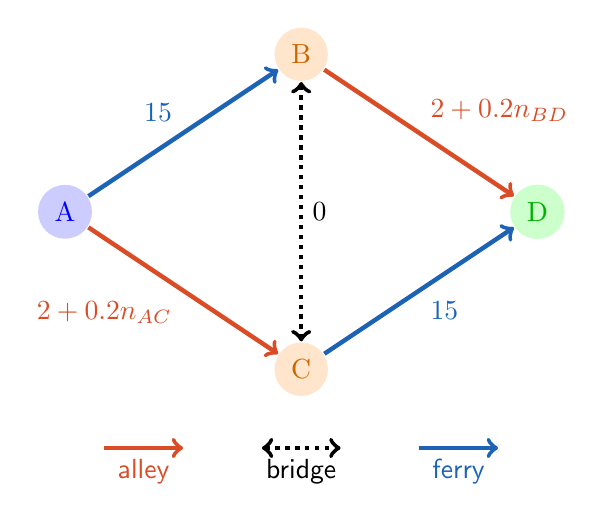
\begin{tikzpicture}
    \node (A) at (0,0) [thick, blue, circle, fill=blue!20] {A};
    \node (D) at (6,0) [thick, green!70!black, circle, fill=green!20] {D};
    \node (B) at (3,2) [thick, orange!80!black, circle, fill=orange!20] {B};
    \node (C) at (3,-2) [thick, orange!80!black, circle, fill=orange!20] {C};

    % ferry
    \draw [->, ultra thick, cyan!40!blue] (A)--(B) node[midway, anchor=south east]{15};
    \draw [->, ultra thick, cyan!40!blue] (C)--(D) node[midway, anchor=north west]{15};

    % alley
    \draw [->, ultra thick, red!40!brown] (A)--(C) node[midway, anchor=north east]{$2+0.2 n_{AC}$};
    \draw [->, ultra thick, red!40!brown] (B)--(D) node[midway, anchor=south west]{$2+0.2 n_{BD}$};

    % bridge
    \draw [<->, dotted, ultra thick] (B)--(C) node[midway,right]{0};

    % legend
    \draw [->, ultra thick, red!40!brown] (0.5,-3)--(1.5,-3) node[midway, anchor = north]{\textsf{alley}};
    \draw [<->, dotted, ultra thick] (2.5,-3)--(3.5,-3) node[midway, anchor = north]{\textsf{bridge}};
    \draw [->, ultra thick, cyan!40!blue] (4.5,-3)--(5.5,-3) node[midway, anchor = north]{\textsf{ferry}};
\end{tikzpicture}
}
\newcommand{\secondgamecosts}{
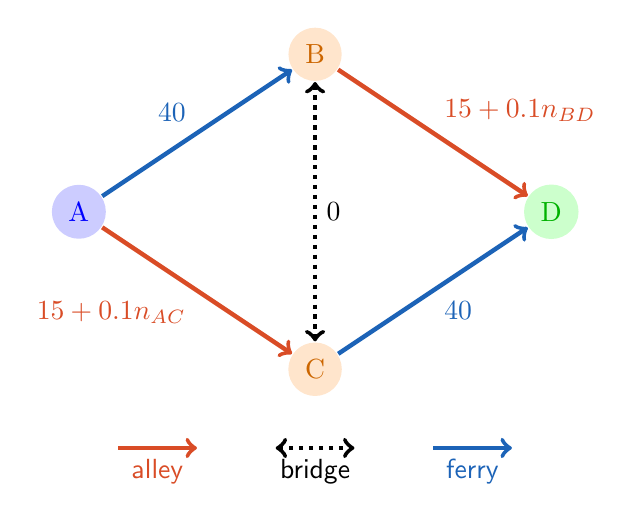
\begin{tikzpicture}
    \node (A) at (0,0) [thick, blue, circle, fill=blue!20] {A};
    \node (D) at (6,0) [thick, green!70!black, circle, fill=green!20] {D};
    \node (B) at (3,2) [thick, orange!80!black, circle, fill=orange!20] {B};
    \node (C) at (3,-2) [thick, orange!80!black, circle, fill=orange!20] {C};

    % ferry
    \draw [->, ultra thick, cyan!40!blue] (A)--(B) node[midway, anchor=south east]{40};
    \draw [->, ultra thick, cyan!40!blue] (C)--(D) node[midway, anchor=north west]{40};

    % alley
    \draw [->, ultra thick, red!40!brown] (A)--(C) node[midway, anchor=north east]{$15+0.1 n_{AC}$};
    \draw [->, ultra thick, red!40!brown] (B)--(D) node[midway, anchor=south west]{$15+0.1 n_{BD}$};

    % bridge
    \draw [<->, dotted, ultra thick] (B)--(C) node[midway,right]{0};

    % legend
    \draw [->, ultra thick, red!40!brown] (0.5,-3)--(1.5,-3) node[midway, anchor = north]{\textsf{alley}};
    \draw [<->, dotted, ultra thick] (2.5,-3)--(3.5,-3) node[midway, anchor = north]{\textsf{bridge}};
    \draw [->, ultra thick, cyan!40!blue] (4.5,-3)--(5.5,-3) node[midway, anchor = north]{\textsf{ferry}};
\end{tikzpicture}
}
\newcommand{\backslashcolor}[2]{\backslashbox{\textcolor{red}{#1}}{\textcolor{blue}{#2}}}


\begin{document}

\begin{frame}

    \titlepage

\end{frame}

\begin{frame}
    \frametitle{Outline}

    \tableofcontents

\end{frame}

\section{What is Braess's Paradox?}

\subsection{Refresher on Game Theory}

\begin{frame}{Game Theory}{A refresher}

    \begin{columns}
    \column[c]{0.7\linewidth}
        
    \begin{block}{}
        Mathematically models interactions between $\underset{\textcolor{gray}{\small (i = 1 \cdots n)}}{\alert<1>{\text{agents}}}$
    \end{block}

    % Include a rock paper scissors game matrix
    \begin{itemize}
        \item<2-> Each agent has a~\only<.>{\textcolor{gray}{finite or infinite }}set of \alert<2>{actions} \structure{$a_i \in \mathcal{A}_i$}
        \item<3-> Tries to maximize their \alert<3>{reward} \structure{$J_i(a_1, \cdots a_n)$}
        \item<4-> If no agent can do better by unilaterally changing their action $a_i$ - \structure{$\{a_1^*, \cdots a_n^*\}$} is a \alert<4->{Nash Equilibrium}
    \end{itemize}
    
    \begin{columns}<5->
        \column{0.4\linewidth}
        \begin{block}{Social Cost}
            \small{indicates the well-being of the society}
            \begin{center}
                \structure{$\sum\limits_{i=1}^{n}J_i(a_1, \cdots a_n)$}
            \end{center}
        \end{block}
        \column{0.4\linewidth}
        \begin{block}{Price of Anarchy} \small
            indicates if the NE cost is better or worse than the lowest achievable cost
        \end{block}
    \end{columns}
    
    \column{0.29\linewidth}
    \begin{center}
    
        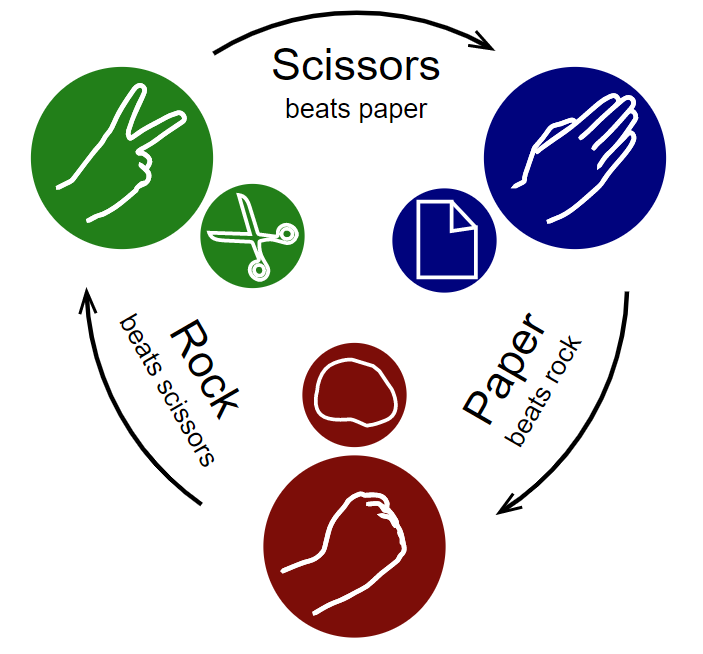
\includegraphics[width=\linewidth]{images/Rock_paper_scissors.png} 
    % https://commons.wikimedia.org/wiki/File:Rock-paper-scissors.svg, Attribution: Enzoklop, CC BY-SA 3.0 <https://creativecommons.org/licenses/by-sa/3.0>, via Wikimedia Commons

    \only<2->{$\downarrow$

    \smallskip
    
    \scalebox{0.47}{
\begin{tabular}{c|c|c|c|}
    \backslashcolor{\only<2->{$a_1$}}{\only<2->{$a_2$}} & \only<2->{Rock} & \only<2->{Paper} & \only<2->{Scissors} \\ \hline
    \only<2->{Rock} & \backslashcolor{\only<3->{0}}{\only<3->{0}} &\backslashcolor{\only<3->{-1}}{\only<3->{1}} & \backslashcolor{\only<3->{1}}{\only<3->{-1}} \\ \hline
    \only<2->{Paper} & \backslashcolor{\only<3->{1}}{\only<3->{-1}} &\backslashcolor{\only<3->{0}}{\only<3->{0}} & \backslashcolor{\only<3->{-1}}{\only<3->{1}} \\ \hline
    \only<2->{Scissors} & \backslashcolor{\only<3->{-1}}{\only<3->{1}} &\backslashcolor{\only<3->{1}}{\only<3->{-1}} & \backslashcolor{\only<3->{0}}{\only<3->{0}} \\ \hline
\end{tabular}}}

    
    \end{center}

    \end{columns}

    % \footnotetext[]{\tiny \url{https://commons.wikimedia.org/wiki/File:Rock-paper-scissors.svg}}
    \only<1>{\let\thefootnote\relax\footnotetext{\tiny \url{https://commons.wikimedia.org/wiki/File:Rock-paper-scissors.svg}}}

\end{frame}

\subsection{A congestion game}

\begin{frame}{Crossing the Grand Canal in Venice}{A congestion game}

    % introduce with an example, the congestion game - add alley/canal image from trip
    \begin{columns}
        \column{0.6\linewidth}
        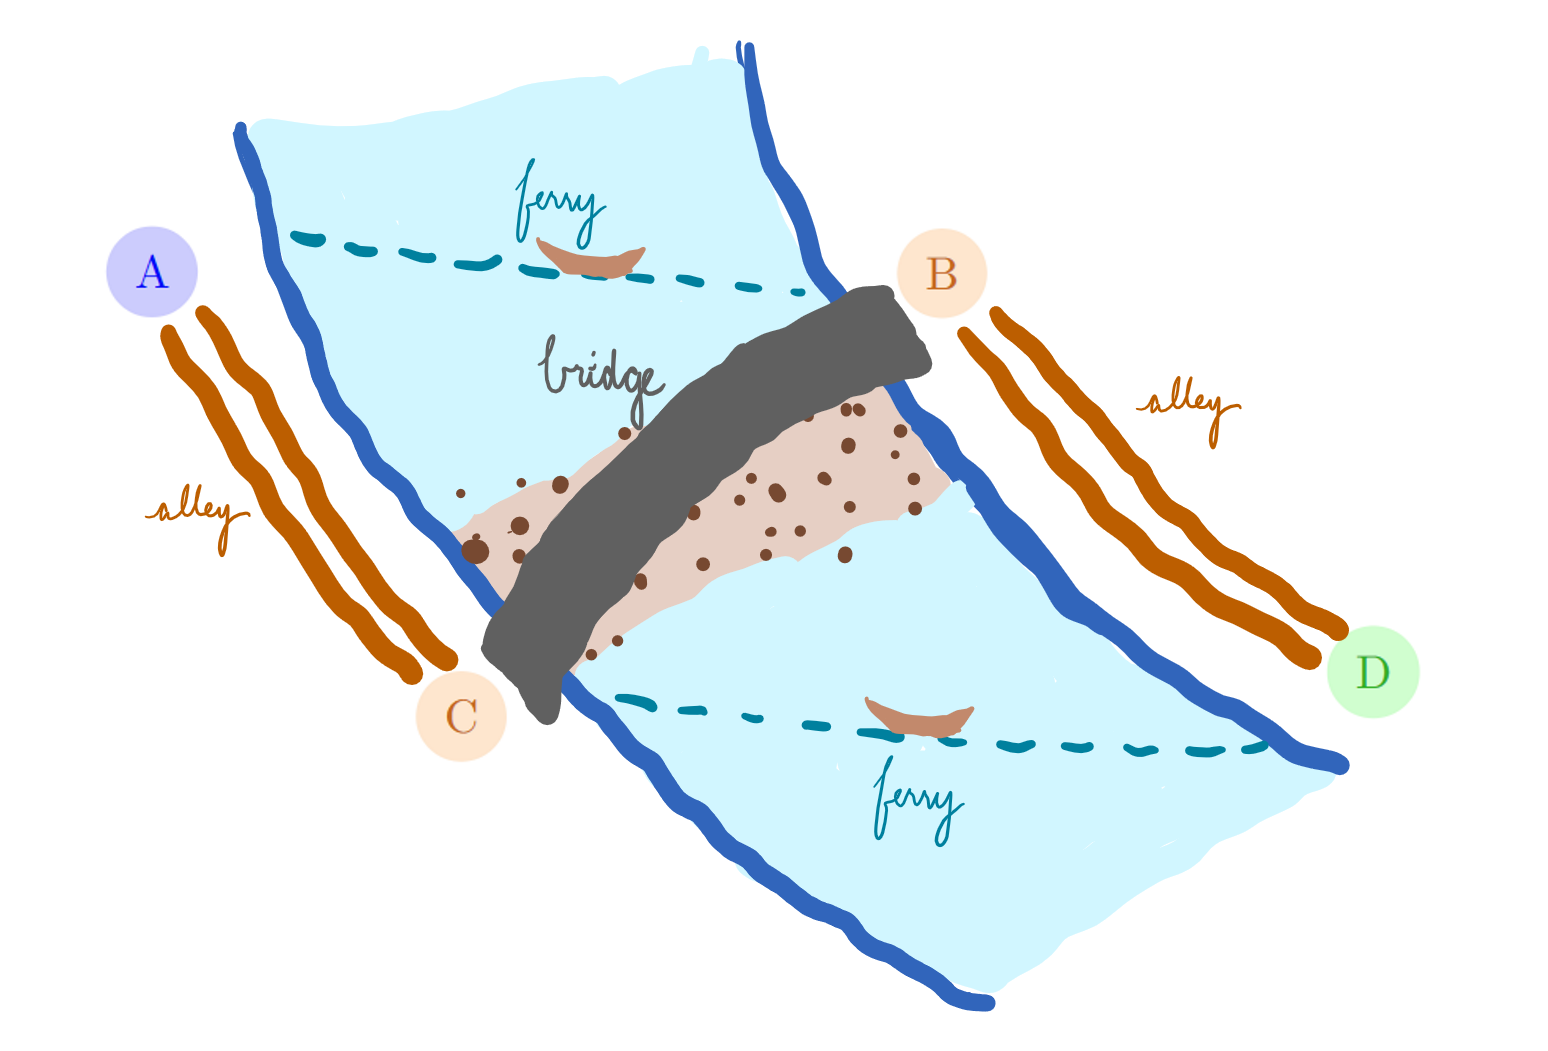
\includegraphics[width=\linewidth]{images/Venice_bridge_crossing_illustration.png}

        \column{0.39\linewidth}
        \begin{center}
            \only<+>{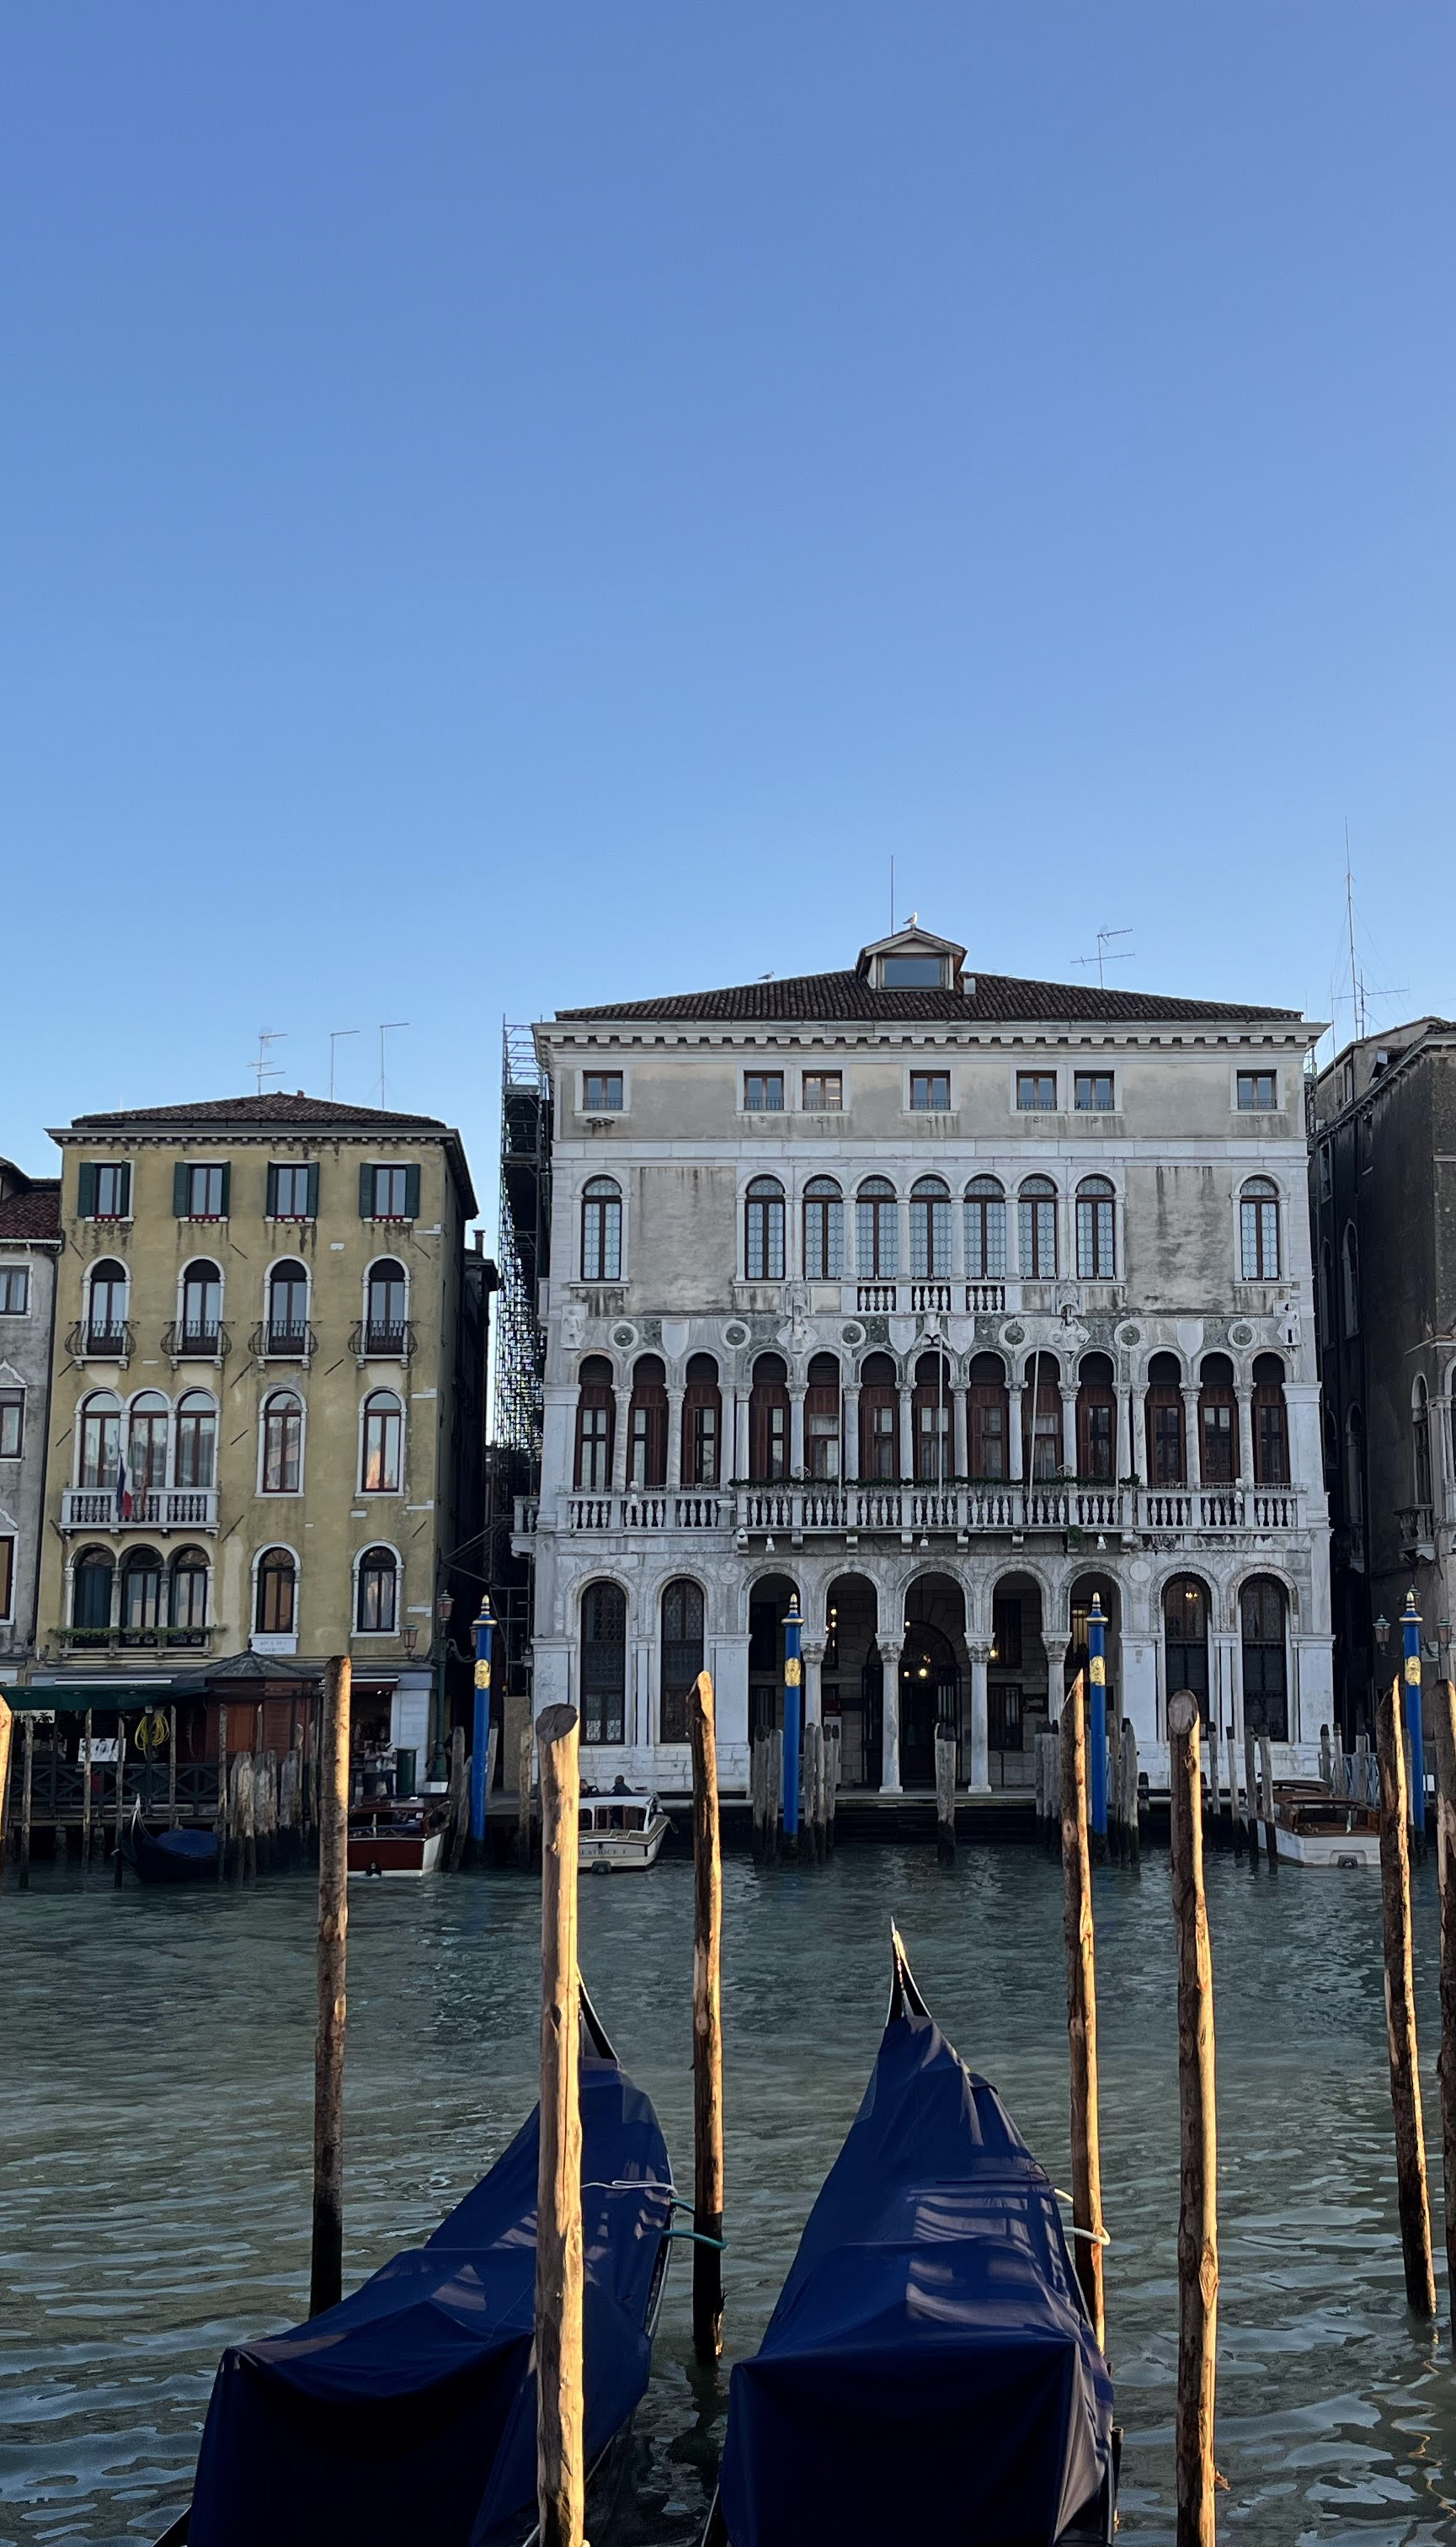
\includegraphics[width=0.7\linewidth]{venice_ferry.jpg}}
            \only<+>{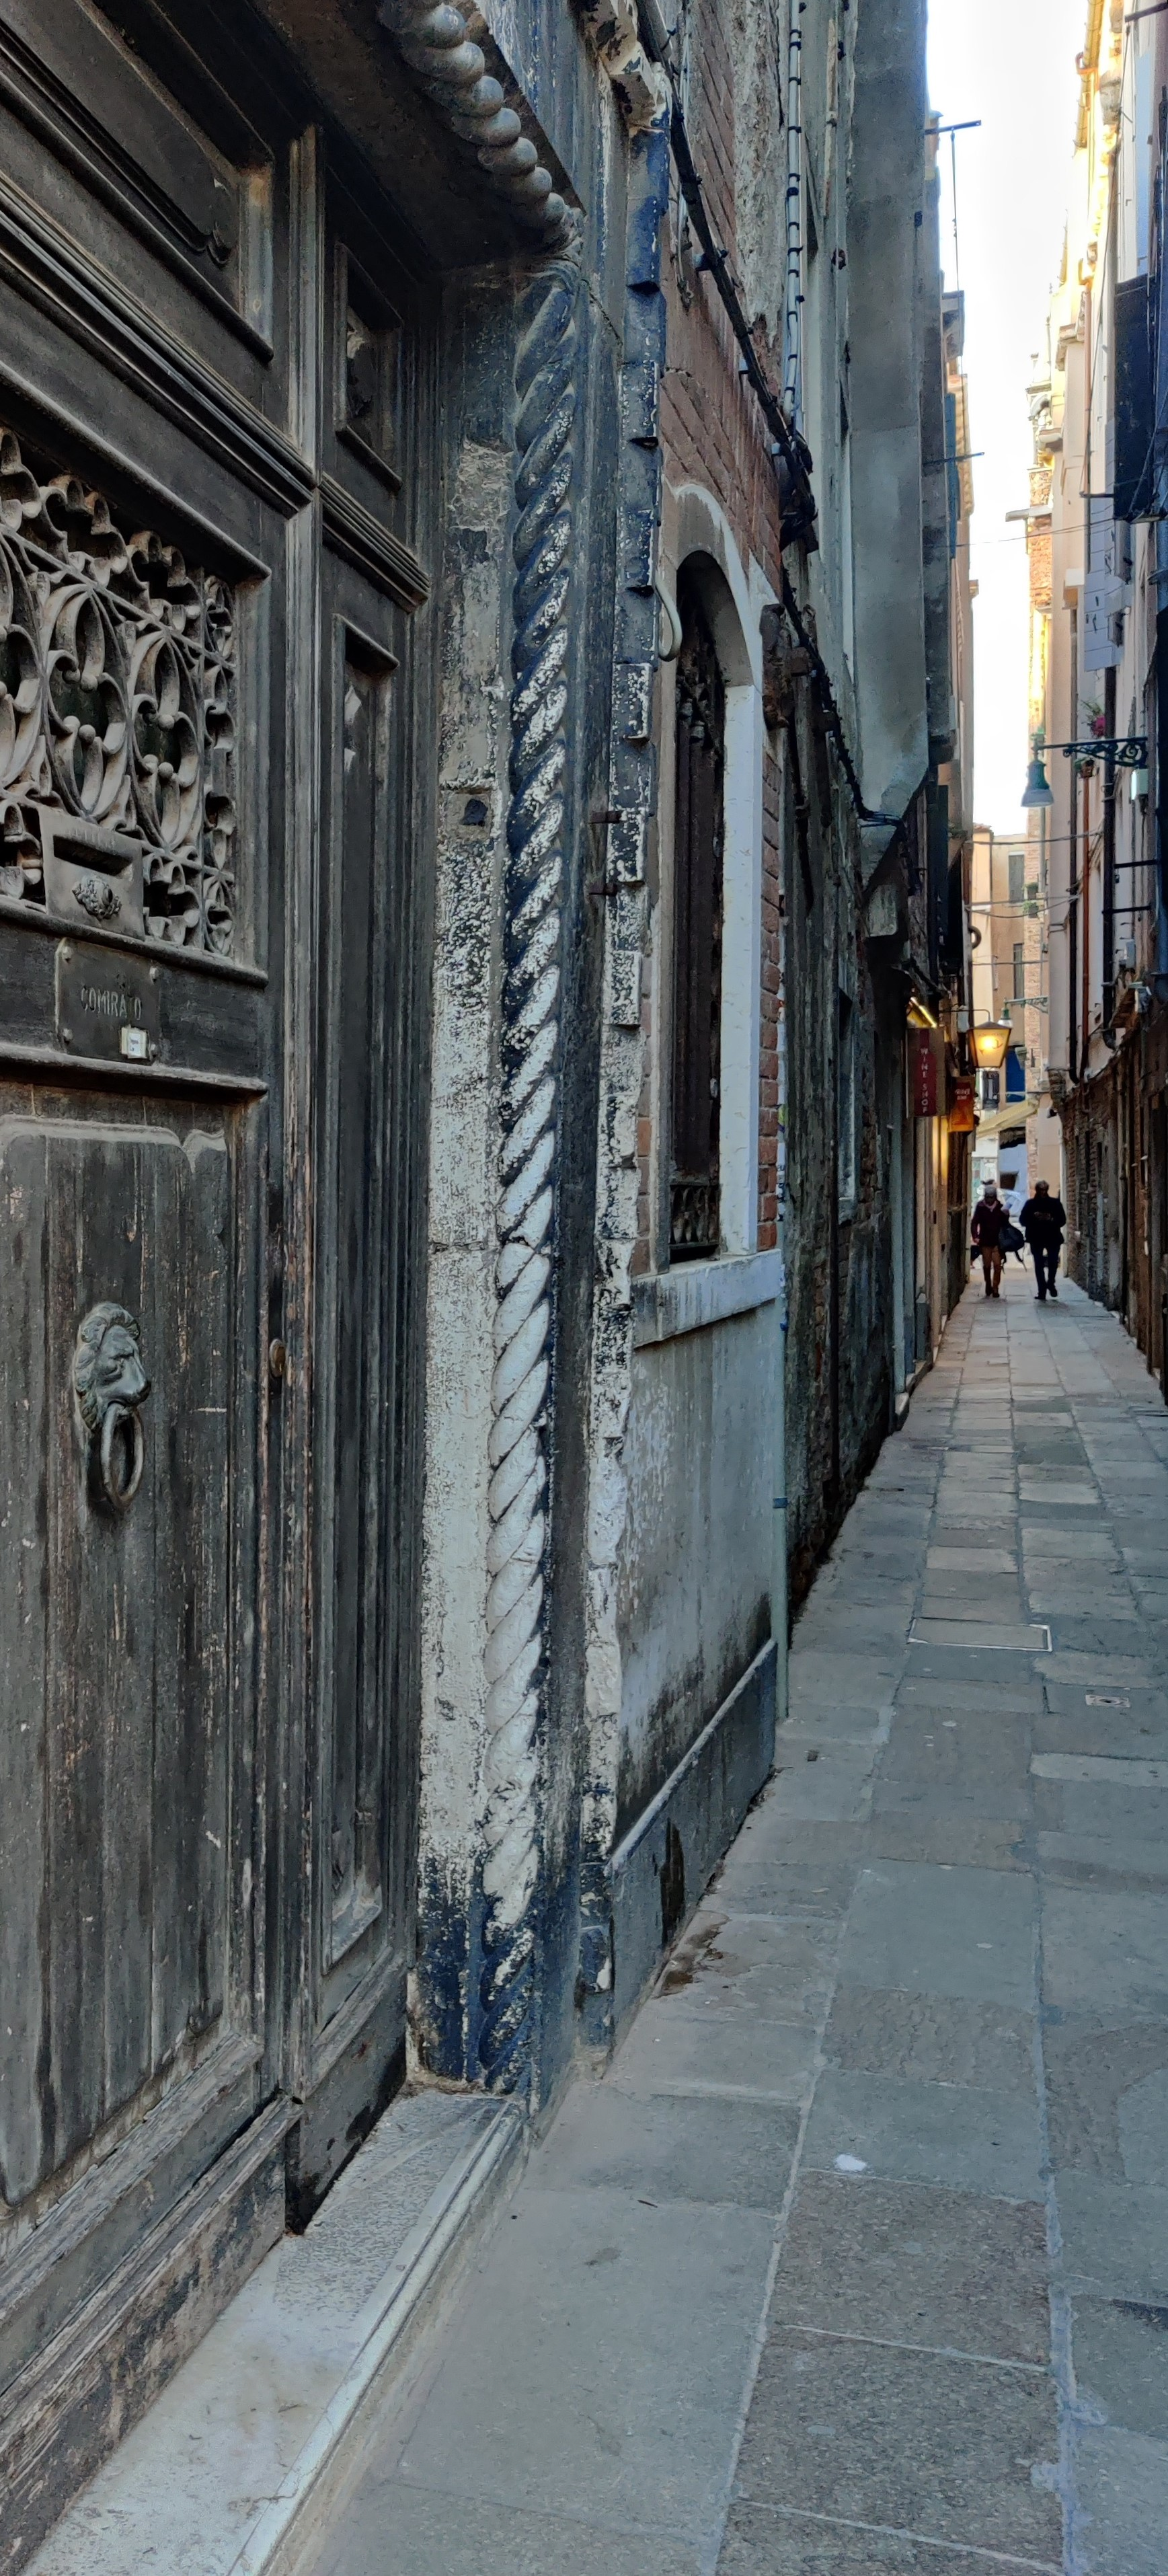
\includegraphics[width=0.55\linewidth]{venice_alley.jpg}
            
            Narrow alleys}
            \only<+>{\scalebox{0.6}{\venicecosts}}
        \end{center}
            
    \end{columns}

\end{frame}

\begin{frame}{Modelling the Game}{Why is it paradoxical?}

    % present game matrix / example numbers and NE solution with and without bridge
        \begin{columns}
        \column{0.55\linewidth}

        \begin{block}<2->{No bridge}
            NE cost: $ 15 + 2 + 0.2\times30 = $ \textbf{23 min}\\  $n_{AC}=n_{BD}=30 $
        \end{block}

        \begin{block}<3->{With bridge}
        
            \begin{tabular}{c|cccc}
                  cost  & ABD & ACD & ABCD & ACBD \\ \hline
                Initial & 23 & 23 & 30 & \textbf<3>{16} \\ 
                \visible<4->{NE & 29 & 29 & 30 & \alert<4>{28}}
            \end{tabular}
            
            \visible<4->{\bigskip \textbf{5 min} increase due to the bridge!}
        \end{block}

        \begin{block}<5->{}
        \begin{center}
            $\text{PoA} = \frac{28}{22.96} =  121.95\%$
        \end{center}
        \end{block}



        \column{0.39\linewidth}
        \begin{center}
            \begin{block}{Time taken}
            \small{
                \textcolor{cyan!40!blue}{Ferry: \textbf{15 min}}

                \textcolor{red!40!brown}{Alley: \textbf{2 min} + \textbf{12 sec} per person}

                Bridge: \faBolt

                \hfill and \textbf{60} agents.
                }
            \end{block}

            \bigskip
            
            {\scalebox{0.6}{\venicecosts}}
        \end{center}
            
    \end{columns}
    
\end{frame}

\begin{frame}{Modelling the Game}{It is not just these numbers...}

    % present game matrix / example numbers and NE solution with and without bridge
        \begin{columns}
        \column{0.55\linewidth}

        \begin{block}{No bridge}
            NE cost: $ 40 + 15 + 0.1\times100 = $ \textbf{65 min}\\  $n_{AC}=n_{BD}=100 $
        \end{block}

        \begin{block}{With bridge}
        
            \begin{tabular}{c|cccc}
                  cost  & ABD & ACD & ABCD & ACBD \\ \hline
                Initial & 65 & 65 & 80 & \textbf{50} \\ 
                NE & 75 & 75 & 80 & \alert{70}
            \end{tabular}
            
            \bigskip \textbf{5 min} increase due to the bridge!
        \end{block}

        \begin{block}{}
        \begin{center}
            
            $\text{PoA} = \frac{70}{64.375} =  108.74\%$
        \end{center}
        \end{block}


        \column{0.39\linewidth}
        \begin{center}
            \begin{block}{Time taken}
            \small{
                \textcolor{cyan!40!blue}{Ferry: \textbf{40 min}}

                \textcolor{red!40!brown}{Alley: \textbf{15 min} + \textbf{6 sec} per person}

                Bridge: \faBolt

                \hfill and \textbf{200} agents.
                }
            \end{block}

            \bigskip
            
            {\scalebox{0.6}{\secondgamecosts}}
        \end{center}
            
    \end{columns}
    
\end{frame}

\section{Overcoming the paradox}

\begin{frame}{Preliminary Agent Model}{Introducing the parameters of each agent}

    % Explain the parameters of the agent gamma, neighbours, interaction
        \begin{columns}
        
        \column{0.45\linewidth}
        \begin{block}{Selfishness $\gamma$}
            \small $\gamma \in [0,1]$ indicates how selfish the agent is.
            \begin{description}
                \item[$\gamma=0$] completely selfish
                \item[$\gamma=1$] completely benevolent
            \end{description}
        \end{block}
        
        \column{0.55\linewidth}
        \begin{block}{Connectivity $\mathcal{N}$}
            \small
            $|\mathcal{N}|$ indicates how well-connected an agent is.
            
            $\mathcal{N}$ comprises of the ``neighbours" of the agent.
        \end{block}
    \end{columns}

    \pause
    
    \begin{block}{Cost}
        \small{The cost that each player is trying to minimize}
        \begin{center}
            \structure{$J_i(a_1, \cdots a_n) =(1-\gamma) C_i(a_1, \cdots a_n) +  \gamma\sum\limits_{l \in \mathcal{N}}C_l(a_1, \cdots a_n)$}
        \end{center}
    \end{block}
    \begin{itemize}
        \item Initially, we consider identical agents with fixed parameters
        \item The agents would be regulated by a centralized scheduler
    \end{itemize}    
\end{frame}

\subsection{The Centralized Scheduler}

\begin{frame}
    \frametitle{The Centralized Scheduler}

    % Present absolute optima, argue lots of info exchange needed to achieve
    \begin{columns}
        \column{0.6\linewidth}
        \begin{itemize}
        \item <1->An entity that would regulate the state of affairs
        \item <2->Its job is two-fold: 
        
        - Decide the $\gamma$ and $|\mathcal{N}|$ values
        
        - Schedule/prioritize the agents based on the cost they incur at every stage of the game
        \end{itemize}
        \uncover<4->{
        \begin{figure}
        \scalebox{0.8}{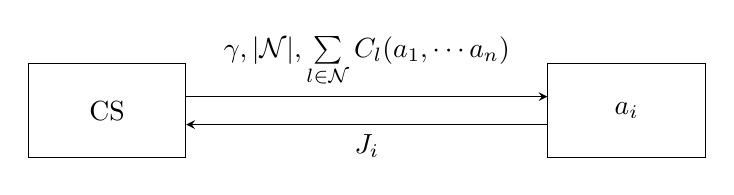
\begin{tikzpicture}
        % CS
        \node [draw,
            minimum width=2cm,
            minimum height=1.2cm,
        ]  (centralscheduler) at (0,0){CS};
         
        % Agent
        \node [draw, 
            minimum width=2cm, 
            minimum height=1.2cm,
        ] (agent) at (6.6,0){$a_i$};

        \draw[-stealth] (centralscheduler.10)--(centralscheduler.10-|agent.west) 
        node[midway,above]{$\gamma,|\mathcal{N}|,     \sum\limits_{l \in \mathcal{N}}C_l(a_1, \cdots a_n)$};
        \draw[-stealth] (agent.-170)--(agent.-170-|centralscheduler.east) 
        node[midway,below]{$J_i$};
        \end{tikzpicture}}
        \caption{Information Exchange}
        \end{figure}}
        
        \column{0.39\linewidth}<3->
        \begin{figure}
        \centering
        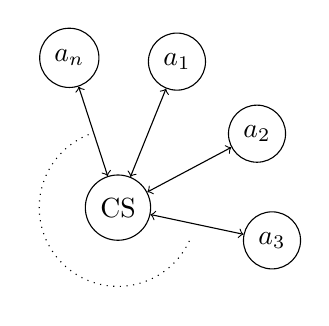
\begin{tikzpicture}
        \label{star_poa}
        \def \n {20}
        \def \N {8}
        \def \radius {2cm}
        \def \rd {1mm}
        \def \rer {4mm}
        
        \def \margin {8} % margin in angles, depends on the radius
        
        \node[draw, circle] at (360:0mm) (ustar) {CS};
        \foreach \i [count=\ni from 0] in {n,1,2,3}{
          \node[draw, circle] at ({108-\ni*40}:\radius) (u\ni) {$a_{\i}$};
          \node at ({115-\ni*40}:\radius/2) {};
          \draw[<->] (ustar)--(u\ni);
        }
        
        \draw[dotted,black] (-25:\radius/2) arc[start angle=-25, end angle=-250, radius=\radius/2];
        \end{tikzpicture}
        \caption{Centralized Scheduler Architecture}
        \end{figure}
            
    \end{columns}
\end{frame}

\begin{frame}{The Centralized Scheduler}{Overall Result}
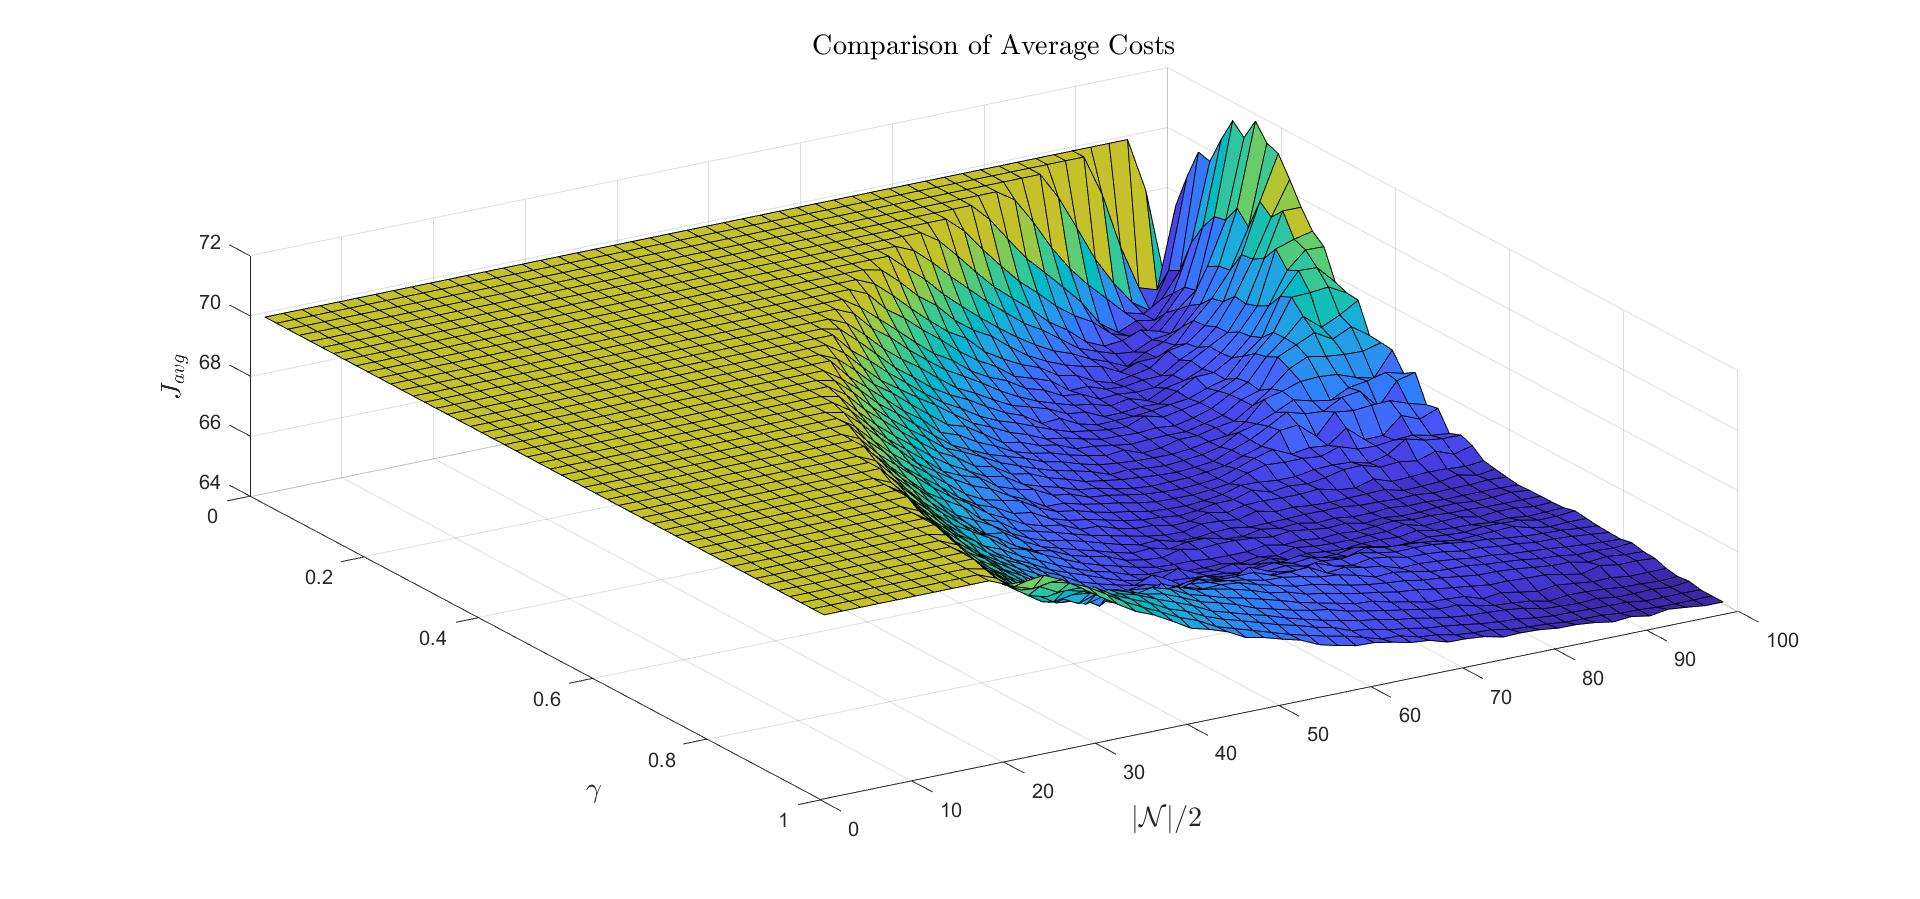
\includegraphics[width=0.9\linewidth]{images/results_central_scheduler_plot.jpg}
\begin{block}{}
            \small{$J_{avg}$ is the \underline{average cost} incurred per agent per stage of the game. The lowest obtained value is 64.375 $<$ 65 for $\gamma =1$ and $|\mathcal{N}|=200$.}
        \end{block}
\end{frame}    
\begin{frame}{The Centralized Scheduler}{Results for $\gamma = 1$ and $|\mathcal{N}|=200$}
\begin{block}{Scheduling}
    The Centralized Scheduler sorts the costs of the different agents after each stage of the game and allows the agents with a high cost to choose their actions early in the next stage. 
\end{block}
\begin{columns}
        \column{0.5\linewidth}
            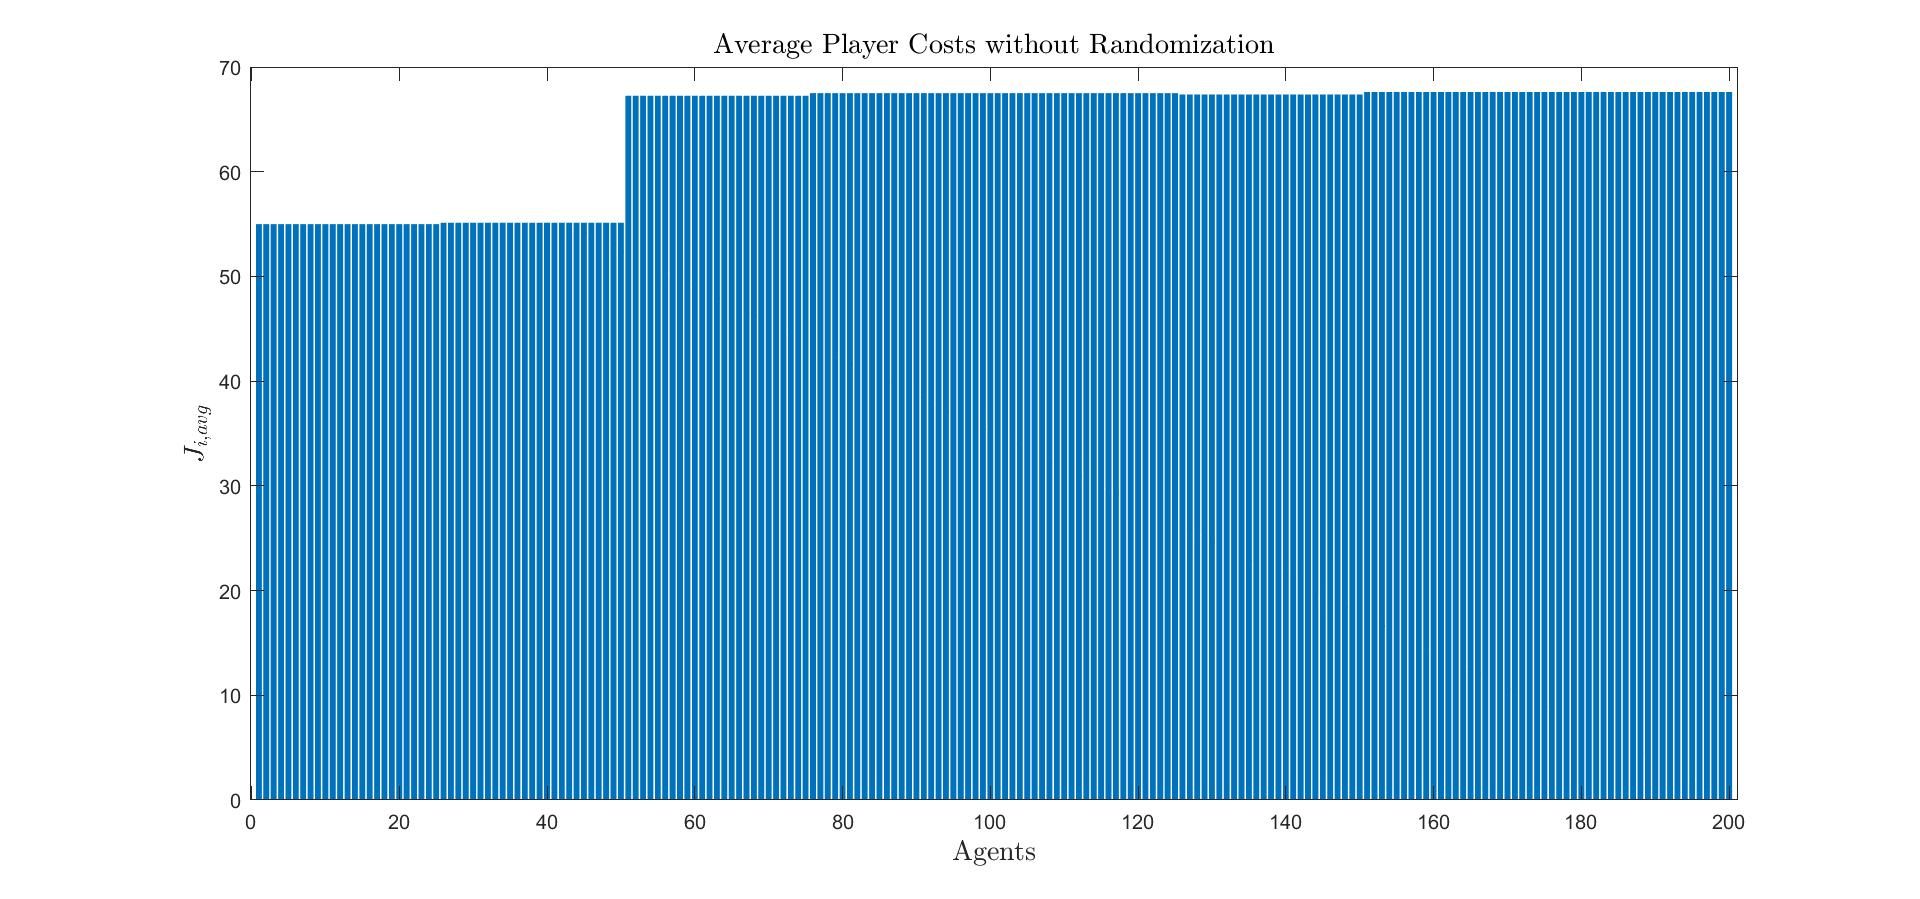
\includegraphics[width=\linewidth, trim={150 0 150 0}, clip]{images/results_central_scheduler_avg_player_no_random.jpg}
        \column{0.5\linewidth}
            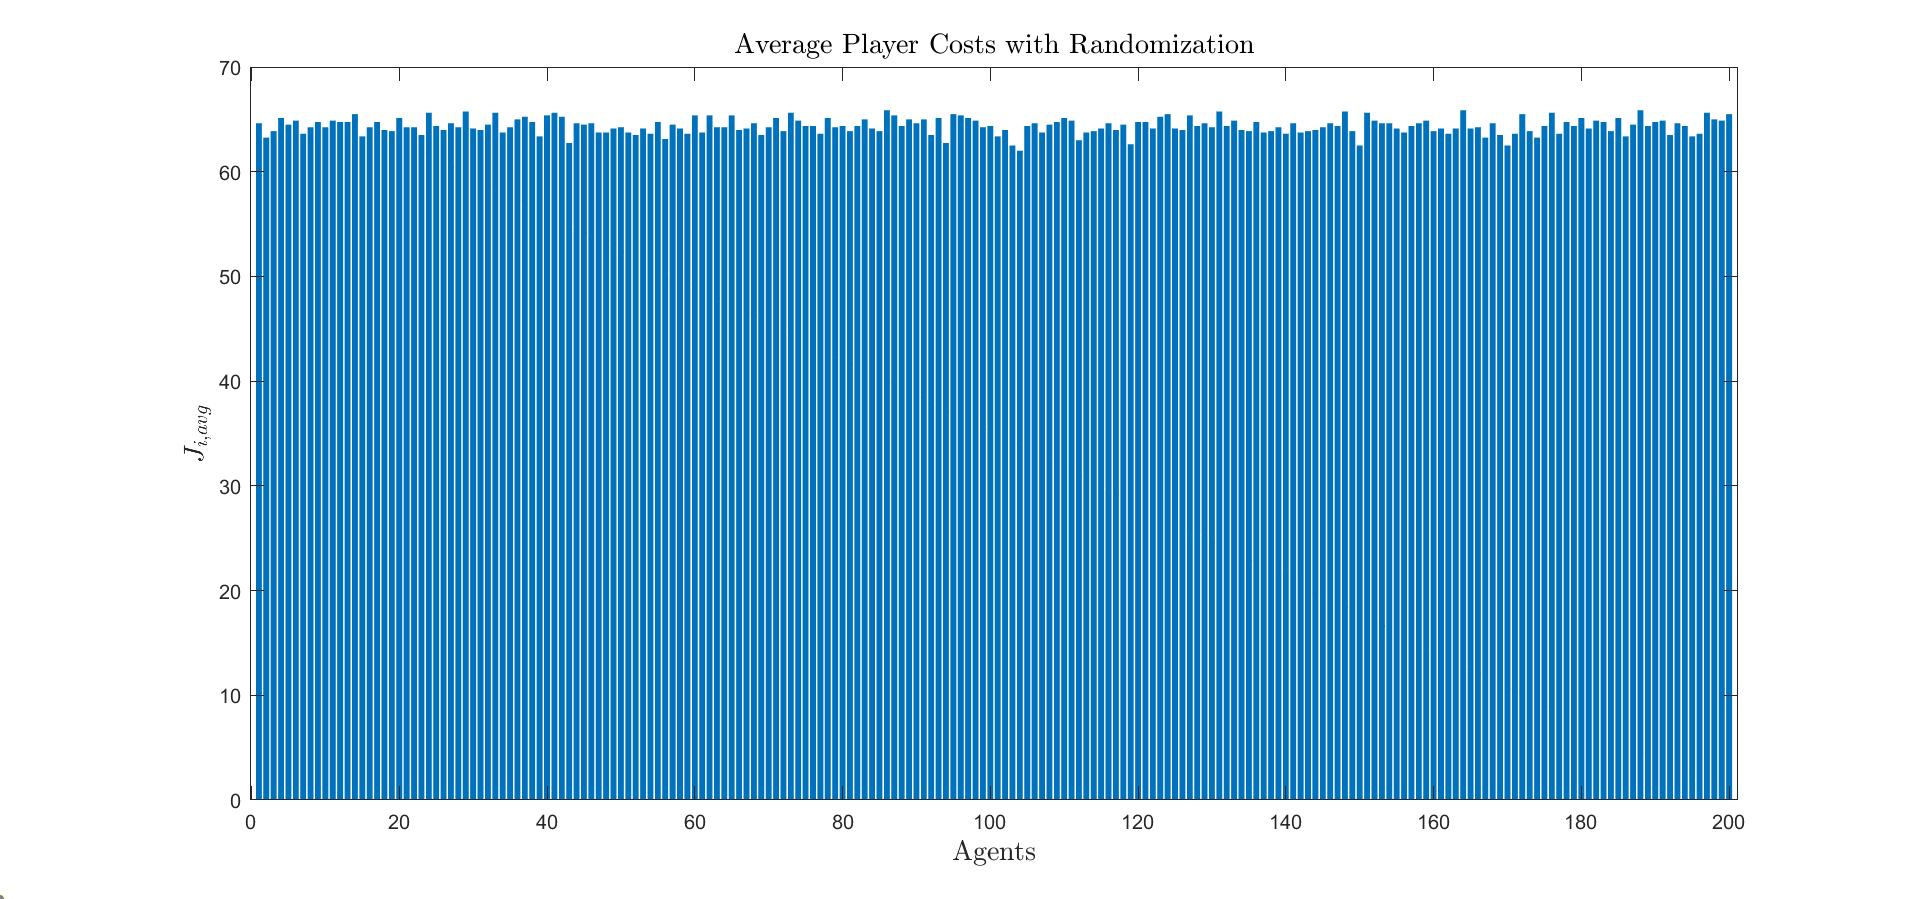
\includegraphics[width=\linewidth, trim={150 0 150 0}, clip]{images/results_central_scheduler_avg_player_random.jpg}
\end{columns}
\begin{block}{}
            $J_{i, \text{avg}}$ is the \underline{average cost} incurred by an agent $i$ over the stages of the game
        \end{block}
\end{frame}

\begin{frame}{The Centralized Scheduler}{What are the problems?}
\begin{itemize}
    \item<1-> May not work out practically
    \item<2-> All decisions are controlled by one entity 
    \item<3-> Does not allow for agents to act independently and choose their own actions
    \item<4-> Rational agents can simply choose to refuse commands from the Scheduler - ``Rogue" Agents
    \item<5-> Limited by the chosen values of $\gamma$ and $|\mathcal{N}|$
\end{itemize}
\end{frame}

\subsection{A Distributed Approach}

\begin{frame}{Dynamic Agent Model}{Introducing dynamics to the parameters of each agent}
\begin{itemize}
    \item<1-> In the absence of a centralized scheduler
    \item<2-> What if the agents decide to update their parameters themselves?
    \item<6-> A "reasonable" agent, self-regulating model 
\end{itemize}
\begin{columns}
\column{0.45\linewidth}
        \begin{block}<3->{Selfishness $\gamma_i(t)$}
            If $J_i(t-1) > \tau$\\
            \quad Be more selfish\\
            Else\\
            \quad Be less selfish\\
        \end{block}
        
        \column{0.5\linewidth}
        \begin{block}<4->{Connectivity $\mathcal{N}_i(t)$}
            If $J_i(t-1) > \tau$\\
            \quad Reduce the number of neighbours\\
            Else\\
            \quad Increase the number of neighbours\\
        \end{block}
    \end{columns}
    \begin{block}<5->{Cost Threshold $\tau$}
    An ``informed" decision of $\tau$ can be made by the agents based on the NE cost they used to incur prior to the construction of the bridge.
    \end{block}
\end{frame}

\begin{frame}{Dynamic Agent Model}{A heuristic dynamic}
\begin{itemize}
    \item In the absence of a centralized scheduler
    \item What if the agents decide to update their parameters themselves?
    \item A "reasonable" agent, self-regulating model 
\end{itemize}
\begin{columns}
\column{0.45\linewidth}
        \begin{block}{Selfishness $\gamma_i(t)$}
            If $J_i(t-1) > \tau$\\
            \quad$\gamma_i(t) = \max(0,\gamma_i(t-1)/4)$\\
            Else\\
            \quad$\gamma_i(t) = \min(1,2\gamma_i(t-1))$\\
        \end{block}
        
        \column{0.45\linewidth}
        \begin{block}{Connectivity $\mathcal{N}_i(t)$}
            If $J_i(t-1) > \tau$\\
            \quad$|\mathcal{N}_i(t)| = \max(0,|\mathcal{N}_i(t-1)|/4)$\\
            Else\\
            \quad$|\mathcal{N}_i(t)| = \min(1,2|\mathcal{N}_i(t-1)|)$\\
        \end{block}
    \end{columns}
    \begin{block}{Cost Threshold $\tau$}
    An ``informed" decision of $\tau$ can be made by the agents based on the NE cost they used to incur prior to the construction of the bridge.
    \end{block}
\end{frame}

\begin{frame}{A Distributed Approach}{Architecture}
\begin{columns}
\column{0.3\linewidth}
\begin{figure}
        \centering
        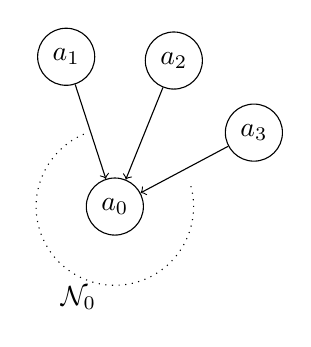
\begin{tikzpicture}
        \label{distributed1}
        \def \n {20}
        \def \N {8}
        \def \radius {2cm}
        \def \rd {1mm}
        \def \rer {4mm}
        
        \def \margin {8} % margin in angles, depends on the radius
        
        \node[draw, circle] at (360:0mm) (ustar) {$a_0$};
        \foreach \i [count=\ni from 0] in {1,2,3}{
          \node[draw, circle] at ({108-\ni*40}:\radius) (u\ni) {$a_{\i}$};
          \node at ({115-\ni*40}:\radius/2) {};
          \draw[<-] (ustar)--(u\ni);
        }
        
        \draw[dotted,black] (15:\radius/2) arc[start angle=15, end angle=-250, radius=\radius/2]
        node[midway,below]{$\mathcal{N}_0$};
        \end{tikzpicture}
        \end{figure}
\column{0.3\linewidth}
\begin{figure}
        \centering
        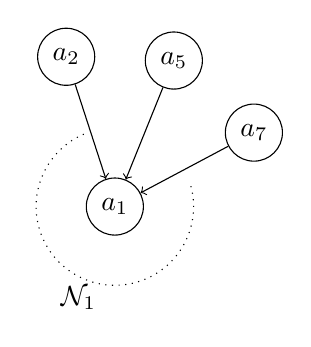
\begin{tikzpicture}
        \label{distributed2}
        \def \n {20}
        \def \N {8}
        \def \radius {2cm}
        \def \rd {1mm}
        \def \rer {4mm}
        
        \def \margin {8} % margin in angles, depends on the radius
        
        \node[draw, circle] at (360:0mm) (ustar) {$a_1$};
        \foreach \i [count=\ni from 0] in {2,5,7}{
          \node[draw, circle] at ({108-\ni*40}:\radius) (u\ni) {$a_{\i}$};
          \node at ({115-\ni*40}:\radius/2) {};
          \draw[<-] (ustar)--(u\ni);
        }
        
        \draw[dotted,black] (15:\radius/2) arc[start angle=15, end angle=-250, radius=\radius/2]
        node[midway,below]{$\mathcal{N}_1$};
        \end{tikzpicture}
\end{figure}
\column{0.05\linewidth}
\dots
\column{0.3\linewidth}
\begin{figure}
        \centering
        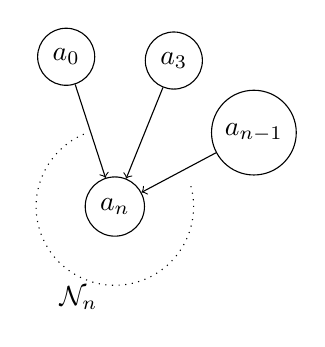
\begin{tikzpicture}
        \label{distributed3}
        \def \n {20}
        \def \N {8}
        \def \radius {2cm}
        \def \rd {1mm}
        \def \rer {4mm}
        
        \def \margin {8} % margin in angles, depends on the radius
        
        \node[draw, circle] at (360:0mm) (ustar) {$a_n$};
        \foreach \i [count=\ni from 0] in {0,3,n-1}{
          \node[draw, circle] at ({108-\ni*40}:\radius) (u\ni) {$a_{\i}$};
          \node at ({115-\ni*40}:\radius/2) {};
          \draw[<-] (ustar)--(u\ni);
        }
        
        \draw[dotted,black] (15:\radius/2) arc[start angle=15, end angle=-250, radius=\radius/2]
        node[midway,below]{$\mathcal{N}_n$};
        \end{tikzpicture}
\end{figure}
\end{columns}
\begin{figure}
        \scalebox{0.8}{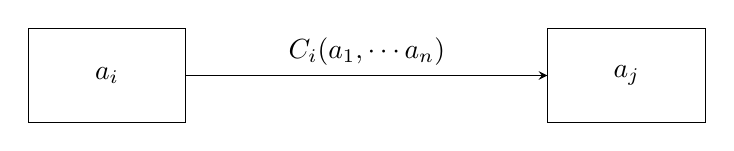
\begin{tikzpicture}
        % a1
        \node [draw,
            minimum width=2cm,
            minimum height=1.2cm,
        ]  (ai) at (0,0){$a_i$};
         
        % a2
        \node [draw, 
            minimum width=2cm, 
            minimum height=1.2cm,
        ] (aj) at (6.6,0){$a_j$};

        \draw[-stealth] (ai.east)--(aj.west) 
        node[midway,above]{$C_i(a_1, \cdots a_n)$};
        \end{tikzpicture}}
        \caption{Information Exchange}
        \end{figure}
\end{frame}
\begin{frame}{A Distributed Approach}{Does it mitigate the shortcomings of the centralized approach?}
\begin{itemize}
    \item<5-> How to implement practically ? - More in Resolution
    \item<1-> \sout{All decisions are controlled by one entity} Each agent has control over their decision
    \item<2-> \sout{Does not allow for agents to act independently and choose their own actions} Every agent acts independently and take their own action
    \item<4-> \sout{Rational agents can simply choose to refuse commands from the Scheduler - "Rogue" Agents} Not applicable, but agents may defect from the said model - More in Resolution 
    \item<3-> \sout{Limited by the chosen values of $\gamma$ and $|\mathcal{N}|$} Agents can choose to update their $\gamma_i(t)$ and $|\mathcal{N}_i(t)|$ values
\end{itemize}
\end{frame}
\begin{frame}{A Distributed Approach}{Results of Monte Carlo Trials with $\gamma_i(0) \sim \mathcal{U}(0,1)$ and $|\mathcal{N}_i(0)| \sim \mathcal{U}(0,200)$}
    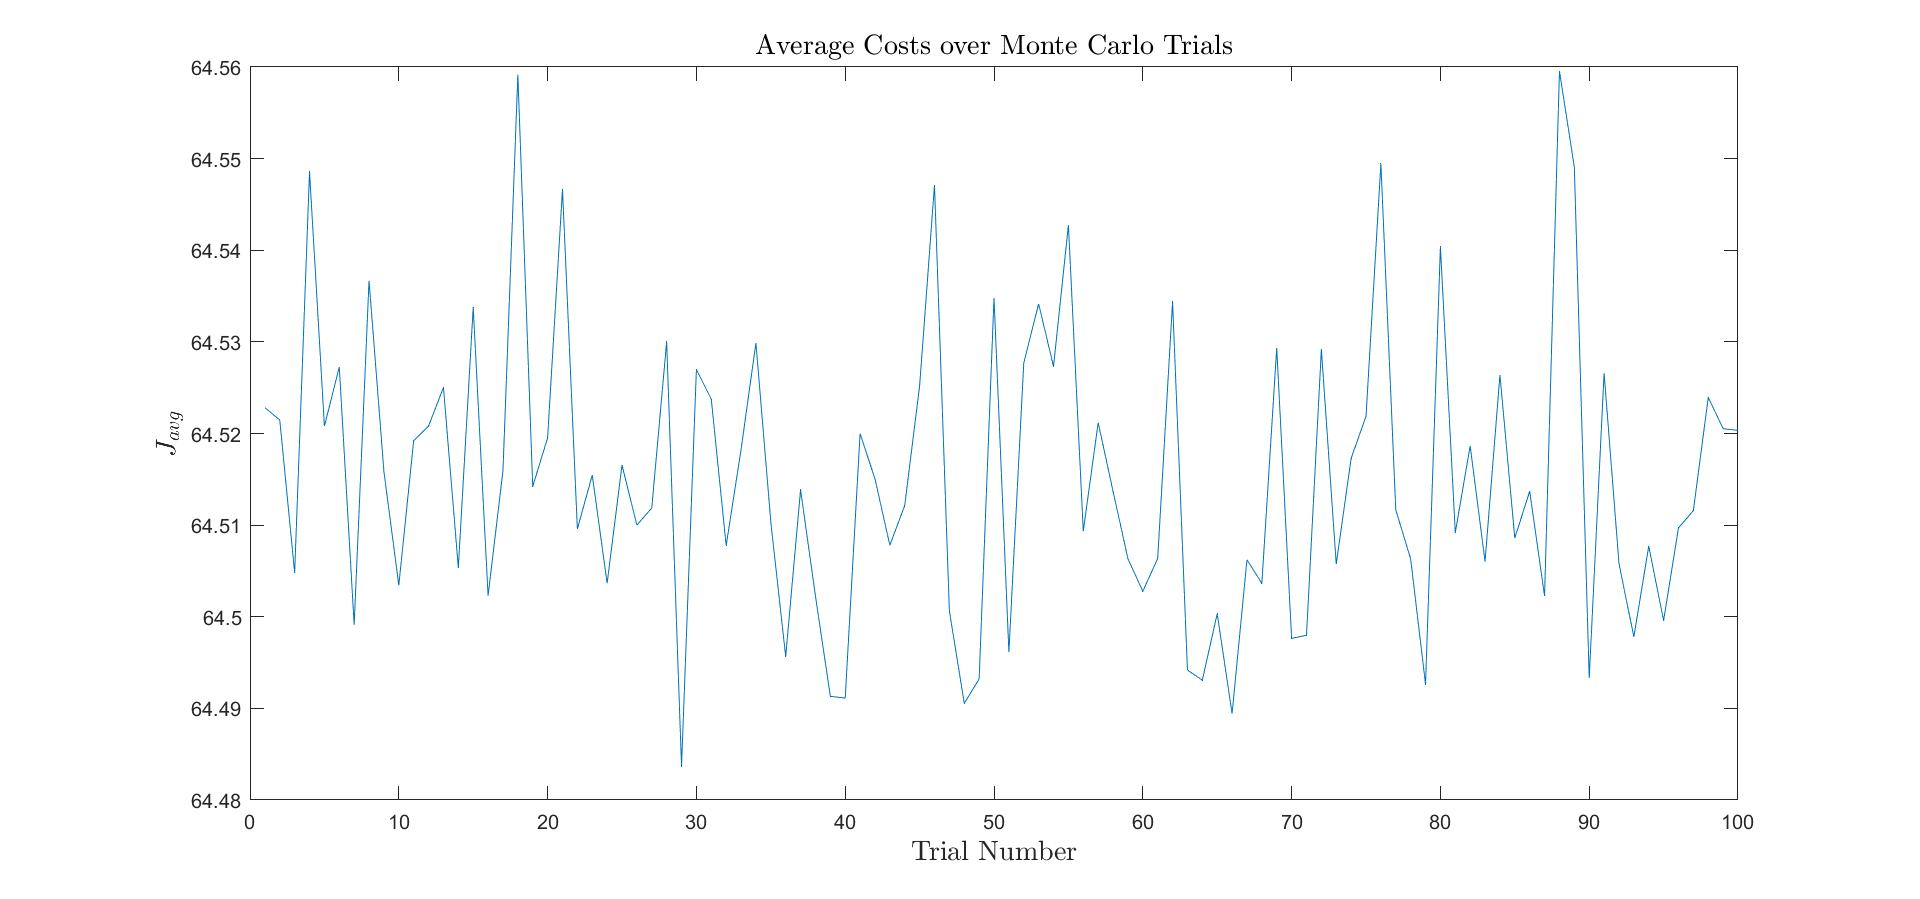
\includegraphics[width=\linewidth]{images/results_distributed_avg_cost.jpg}
    \begin{block}<2->{}
        $J_{avg} \sim \mathcal{N}(64.515, 0.016)$
    \end{block}
\end{frame}

\begin{frame}{A Distributed Approach}{Results of Monte Carlo Trials with $\gamma_i(0) \sim \mathcal{U}(0,1)$ and $|\mathcal{N}_i(0)| \sim \mathcal{U}(0,200)$}
    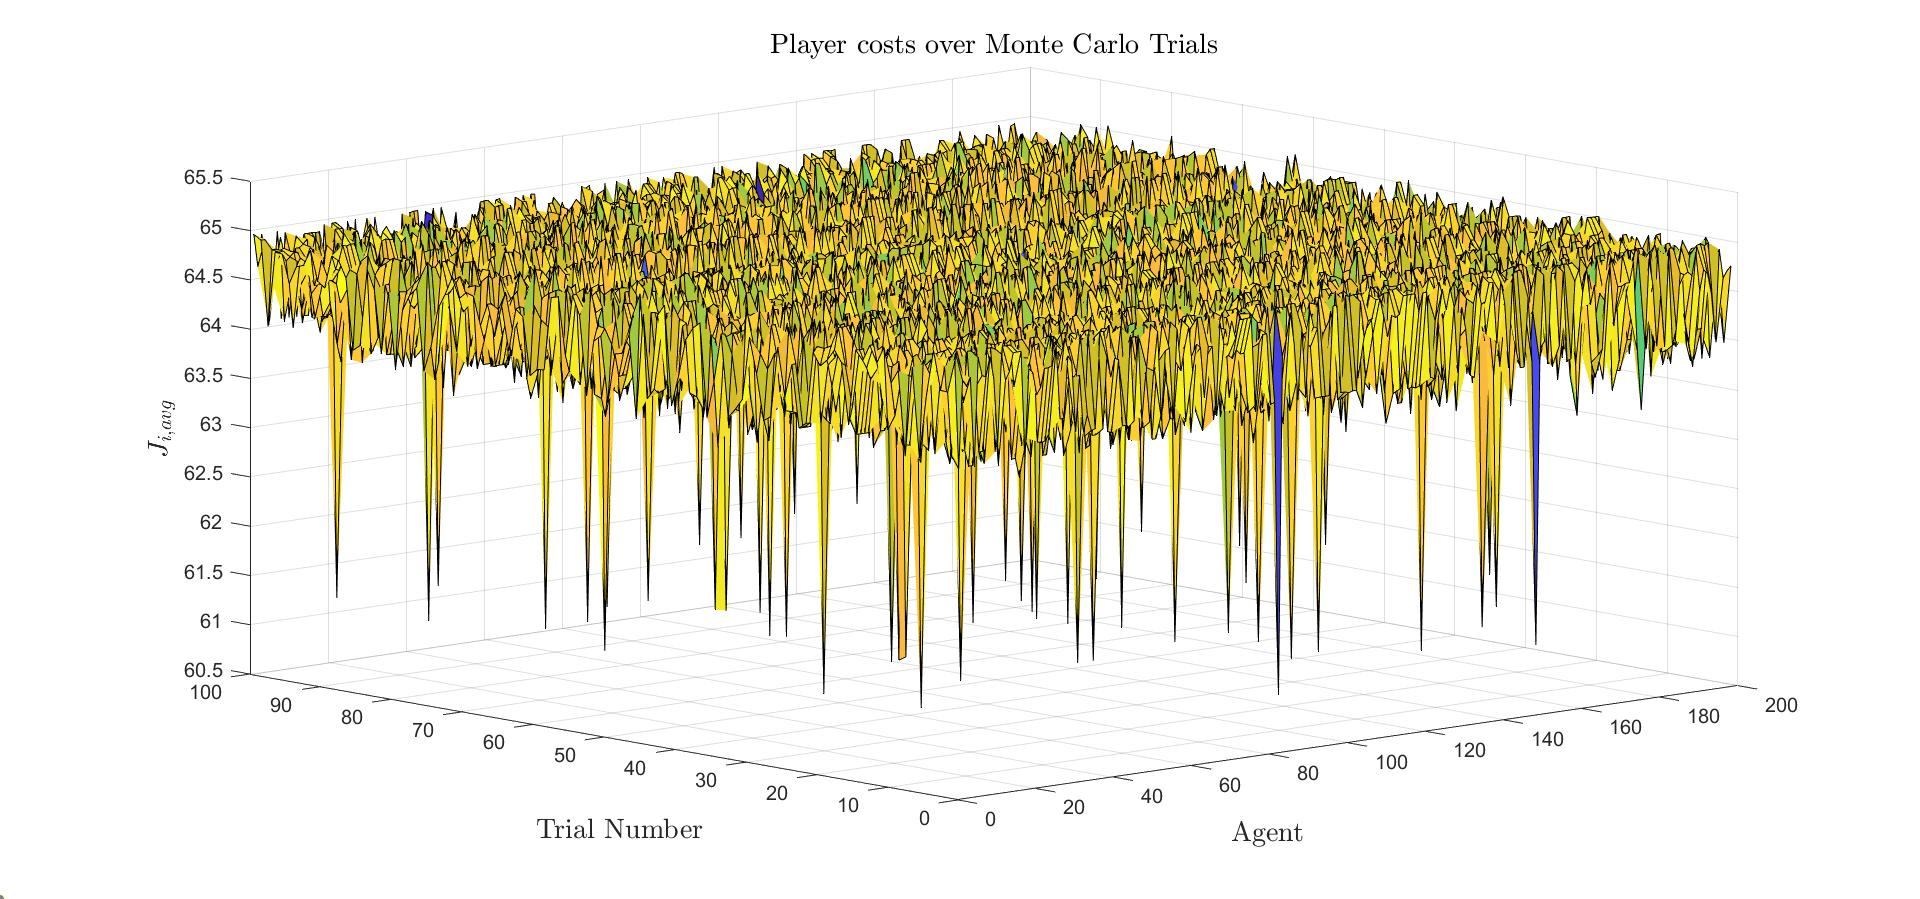
\includegraphics[width=\linewidth]{images/results_distributed_avg_player_cost.jpg}
\end{frame}

\begin{frame}{A Distributed Approach}{Individual Player Parameter Behaviour with $\gamma_i(0) \sim \mathcal{U}(0,1)$ and $|\mathcal{N}_i(0)| \sim \mathcal{U}(0,200)$}
\begin{columns}
\column{0.5\linewidth}
\begin{figure}
    \centering
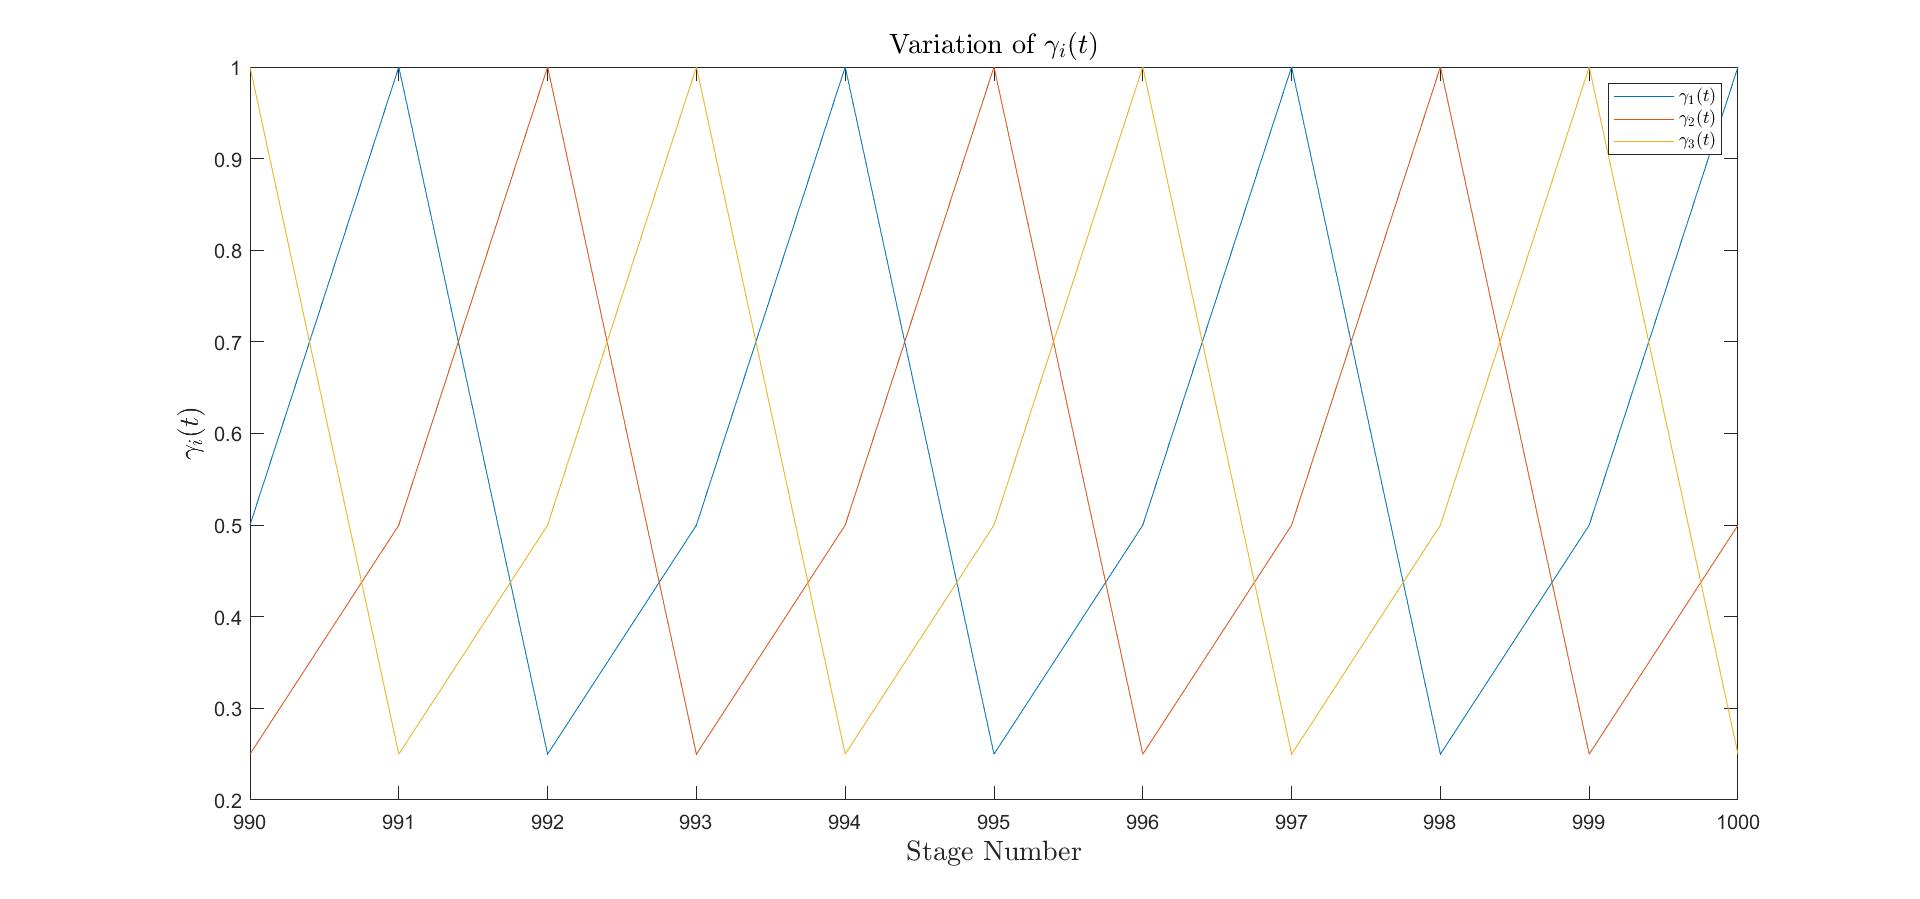
\includegraphics[width=\linewidth]{images/results_distributed_player_gamma.jpg}
    \caption{Variation of $\gamma$ with stage}
\end{figure}
\column{0.5\linewidth}
\begin{figure}
    \centering
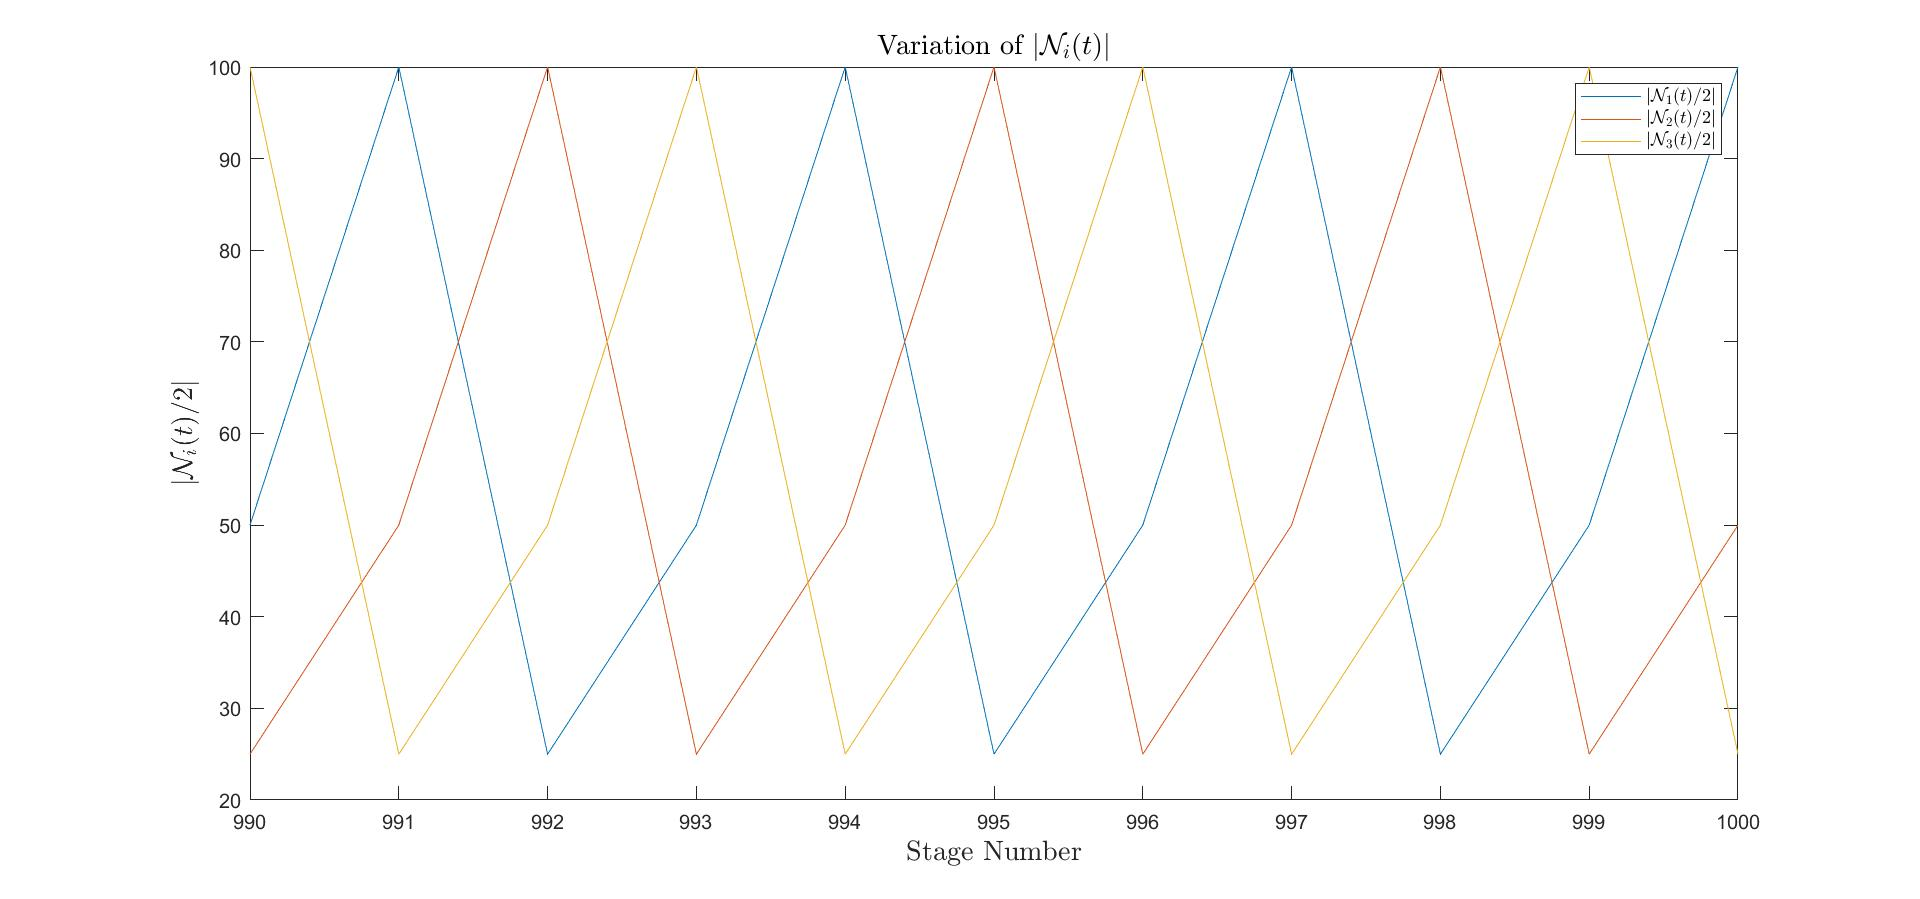
\includegraphics[width=\linewidth]{images/results_distributed_player_neighbours.jpg}
    \caption{Variation of $|\mathcal{N}|$ with stage}
\end{figure}
\end{columns}
\begin{itemize}
    \item <2-> Only a few distinct types of agents, number varies based on their initial parameters
    \item <3-> A ``Limit Cycle" convergence behaviour
    \item <4-> Value of convergence differs with the heuristic chosen to update the parameters of the agents
    
\end{itemize}
\end{frame}
\begin{frame}{A Distributed Approach}{Individual Player Cost Behaviour with $\gamma_i(0) \sim \mathcal{U}(0,1)$ and $|\mathcal{N}_i(0)| \sim \mathcal{U}(0,200)$}
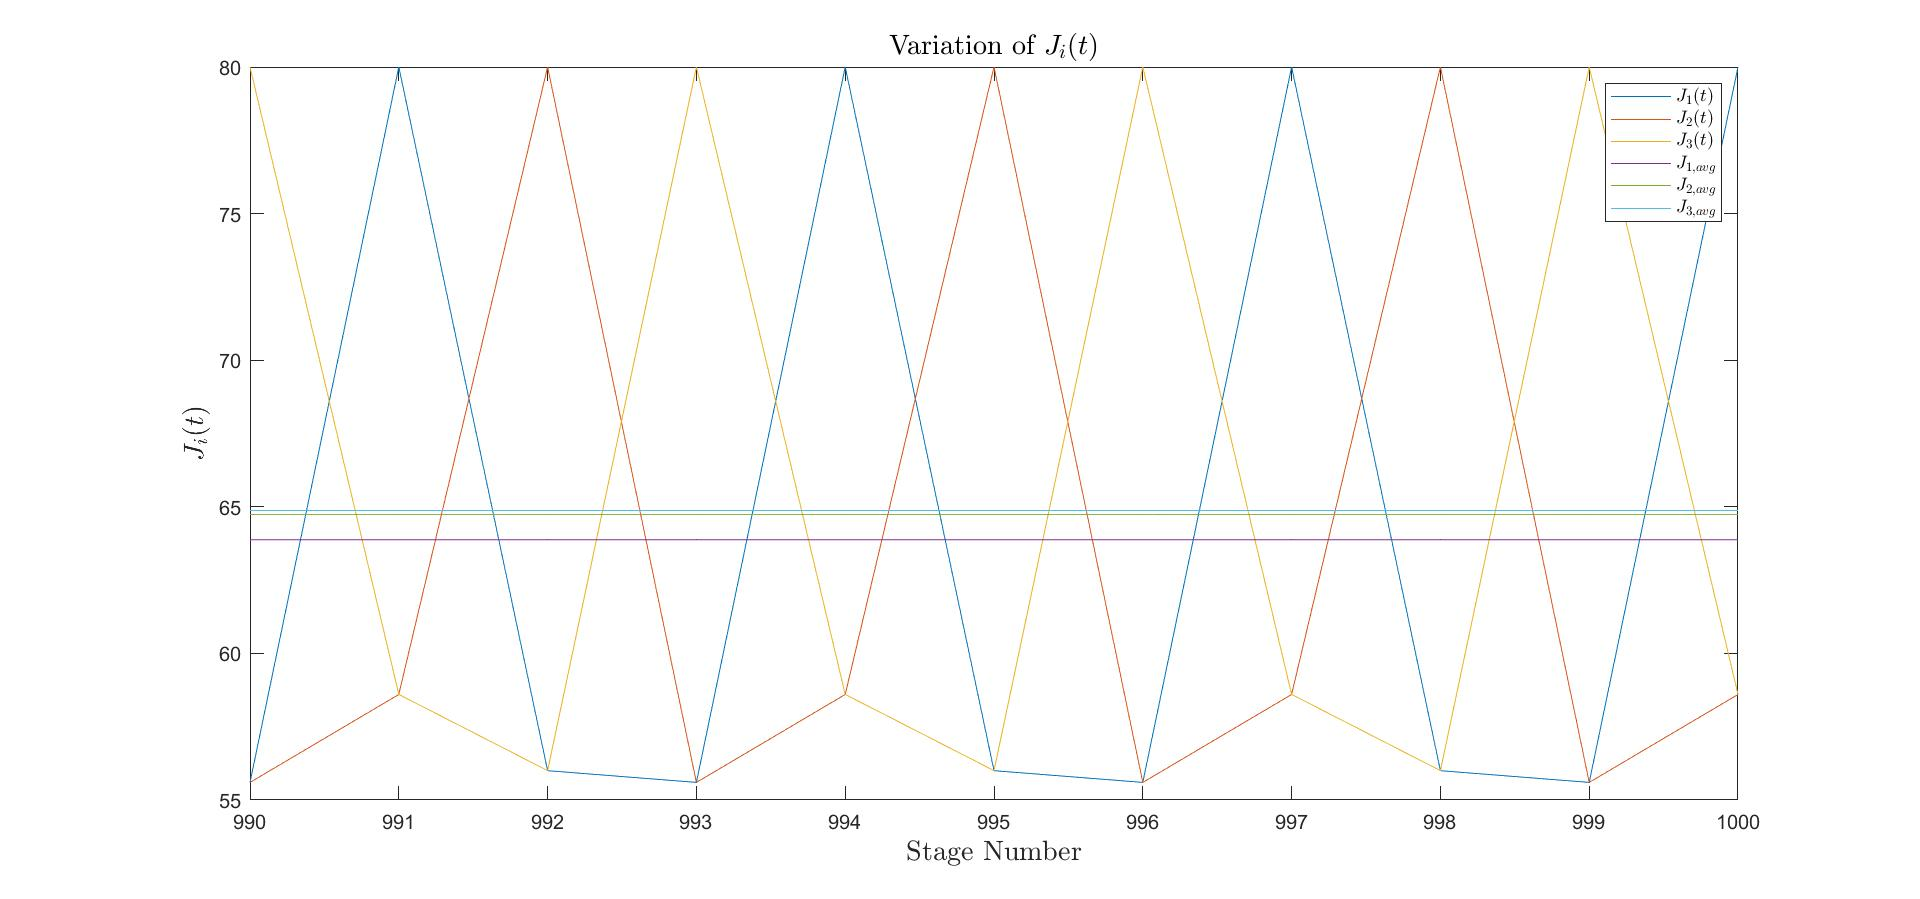
\includegraphics[width=\linewidth]{images/results_distributed_player_cost.jpg}
\end{frame}


\section{Resolution}

\subsection{Conclusion and Outlook}
\begin{frame}{Conclusion}
    % mention PoA, social cost ...

    % mention what we achieved

    % how google Maps can incorporate this

    % remove pic if no space

    \begin{columns}
        \column{0.65\linewidth}
        
        \begin{itemize}
            \item<+-> So did we overcome Braess's Paradox? 
            
            - \textcolor{gray}{Yes, on average in an infinitely repeated game}
            
            \item<+-> Does the bridge actually improve traffic? 
            
            - \textcolor{gray}{Only if agents do not play selfishly }
            
            \item<+-> What would be the practical considerations? 
            
            - \textcolor{gray}{Dynamic agent model might not work with humans, but apps like \structure{Google Maps} or \structure{Apple Maps} can }
        \end{itemize}

        \column{0.3\linewidth}
            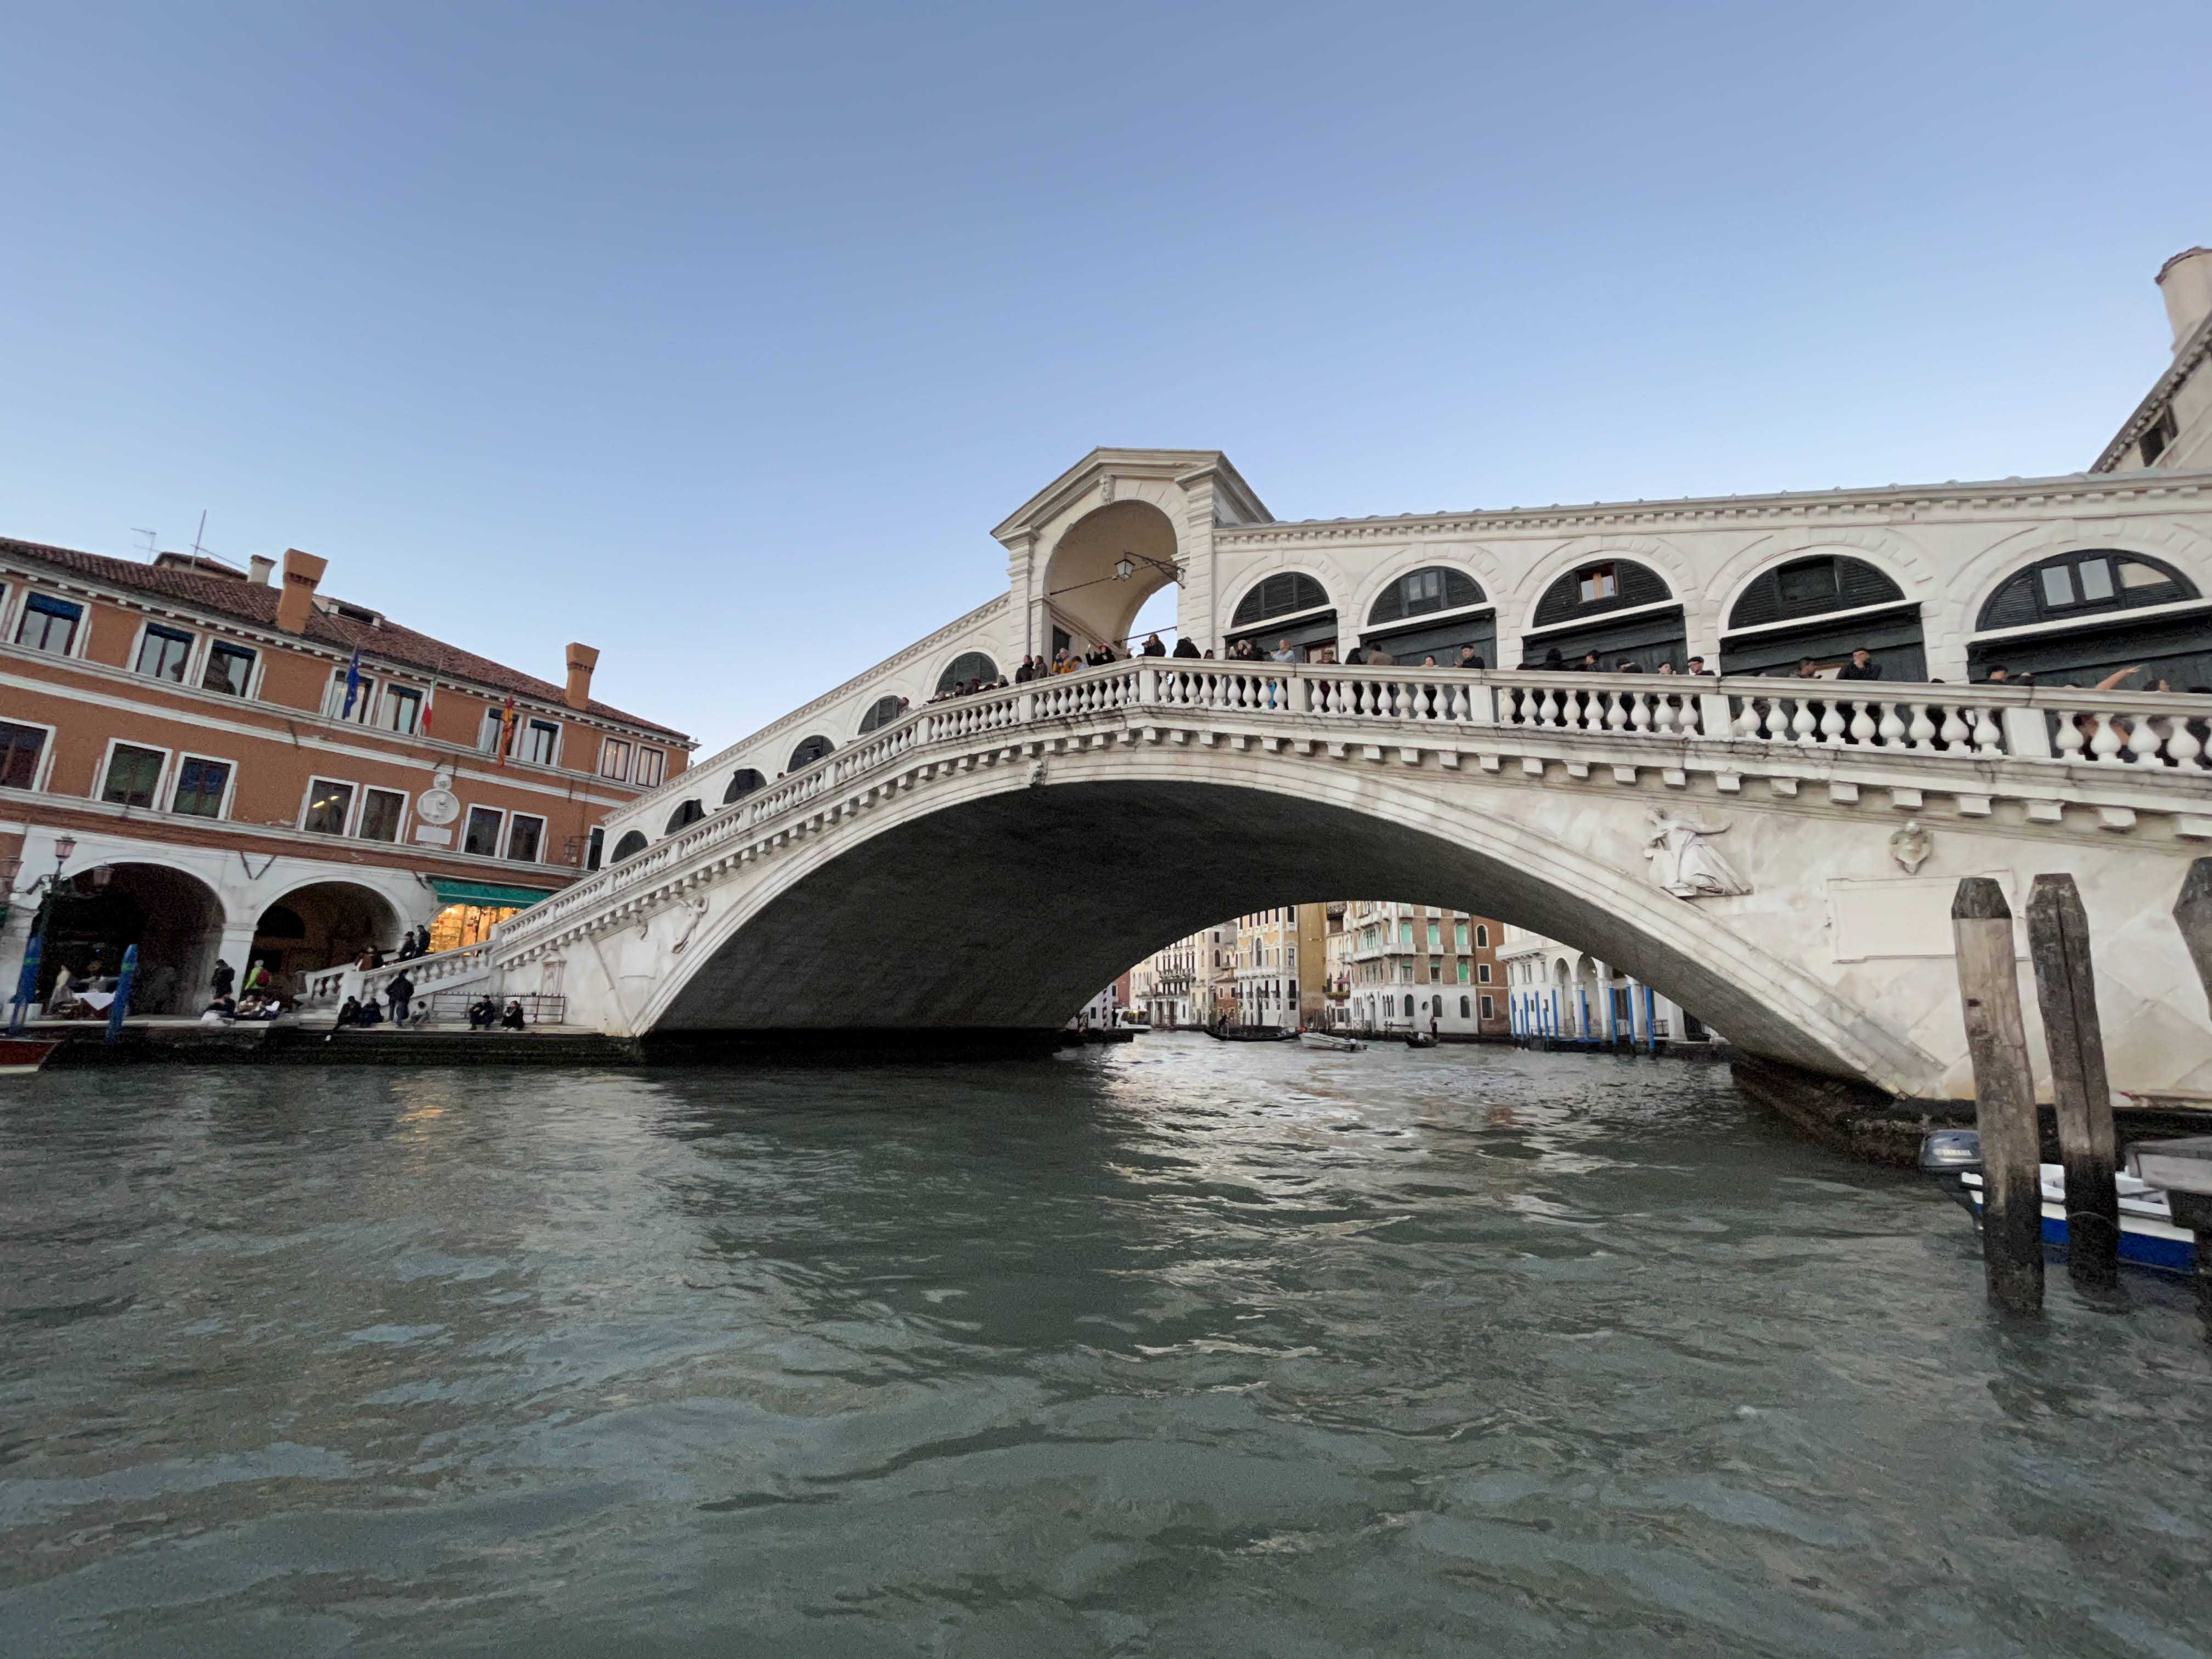
\includegraphics[width=\linewidth]{images/venice_bridge.jpg}
    \end{columns}
   
\end{frame}

\begin{frame}{Outlook}{What's Next?}
\begin{itemize}
    \item<+-> What if the agents are not all ``reasonable" but \structure{some turn selfish} after a few stages of the game? How can the effect be mitigated?
    \item<+-> Can the \structure{heuristics to update the parameters} of the agents be made better?
    \item<+-> The notion of ``intelligent" agents - Can the agents be modelled as neural networks or ML-based entities such that \structure{they learn to be benevolent}?
\end{itemize}
\end{frame}

\subsection{Applications}

\begin{frame}{An example}{... in real life}
\centering

    
\includegraphics[width=0.6\linewidth]{images/42d street NY Times.png}

\bigskip

\begin{quote}
\small
    ``ON Earth Day this year, New York City's Transportation Commissioner \underline{decided to close 42d Street}, which as every New Yorker knows is always congested. ... But to everyone's surprise, Earth Day generated no historic traffic jam. \structure{Traffic flow actually improved when 42d Street was closed.}'' \cite{nytimes}
\end{quote}
% https://www.nytimes.com/1990/12/25/health/what-if-they-closed-42d-street-and-nobody-noticed.html
    
\end{frame}

% \section*{References}

% \begin{frame}{References}

%     \bibliographystyle{unsrt}
%     \bibliography{References}
    
% \end{frame}

\begin{frame}[allowframebreaks]{References}
    
    \begin{thebibliography}{}
        \small
        
        \setbeamertemplate{bibliography item}[book]
        
        \bibitem{Hespanha}
        Hespanha, João P.
        \newblock \emph{Noncooperative Game Theory: An Introduction for Engineers and Computer Scientists. Princeton University Press, 2017.}
        \newblock \url{https://doi.org/10.2307/j.ctt1vwmgbh}.

        \setbeamertemplate{bibliography item}[article]

        \bibitem{Braess}
        Braess, Dietrich, et al. 
        \newblock \emph{``On a Paradox of Traffic Planning.” Transportation Science, vol. 39, no. 4, 2005, pp. 446–450. JSTOR} \newblock \url{http://www.jstor.org/stable/25769266}.
        
        \bibitem{DH}
        Helbing, Dirk, Martin Schönhof, Hans-Ulrich Stark, and Janusz A. Hołyst.
        \newblock How individuals learn to take turns: Emergence of alternating cooperation in a congestion game and the prisoner's dilemma.
        \newblock \emph{Advances in Complex Systems}, 8, no. 01 (2005): 87-116.

        \bibitem{Selfish}
        Tim Roughgarden and Éva Tardos. 2002. H
        \newblock \emph{How bad is selfish routing? J. ACM 49, 2 (March 2002), 236–259.} \newblock \url{https://doi.org/10.1145/506147.506153}


        \setbeamertemplate{bibliography item}[online]

        \bibitem{nytimes}
        Kolata, Gina. 
        \newblock \emph{What if They Closed 42d Street and Nobody Noticed?}, The New York Times, Dec.~25, 1990
        \newblock {\tiny \url{https://www.nytimes.com/1990/12/25/health/what-if-they-closed-42d-street-and-nobody-noticed.html} \small}

        \setbeamertemplate{bibliography item}[triangle]

        \bibitem{bolognani}
        Bolognani, Saverio.
        \newblock \emph{Lecture slides of Game Theory and Control.}
        \newblock Institute for Automatic Control, ETH Z\"urich, Spring 2022.

    \end{thebibliography}
    \vfill
\begin{center}
    
    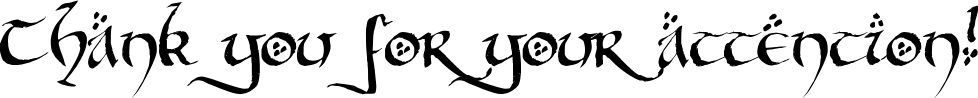
\includegraphics[width=0.5\linewidth]{images/thank_you.png}
\end{center}
    
    \vfill
    
    \hfill \textcolor{gray}{\textit{\footnotesize Images of Venice by authors, Nov 2022.}}
\end{frame}

\end{document}